\documentclass[12pt,letterpaper]{article}

\usepackage{amsmath, amsthm}
\usepackage{microtype, parskip}
\usepackage[comma,numbers,sort&compress]{natbib}
\usepackage{lineno}
\usepackage{docmute}
\usepackage{caption, subcaption, multirow, morefloats, rotating}
\usepackage{wrapfig}

\frenchspacing

\begin{document}

\section*{Results}

Posterior results take one of two forms: direct inspection of parameter estimates, and downstream estimates of diversity and diversification rates. For the former, both the pure-presence and birth-death models (Eq. \ref{eq:pure_presence}, and \ref{eq:birth_death} are inspected. For the latter, only posterior estimates from the birth-death model are considered; the reason for this is explained below in the comparison of the models' posterior predictive check results.

\subsection*{Comparing parameter estimates from the pure-presence and birth-death models}

% look at the posterior predictive checks
%   which model has better fit
%   what does that mean?

Comparison of the posterior predictive performance of the pure-presence and birth-death models reveals a striking difference in quality of the models' fits to the data (Fig. \ref{fig:ppc_pure_presence} and \ref{fig:ppc_birth_death}). The birth-death model is clearly able to reproduce the observed average number of occurrence, in contrast to the pure-birth model which greatly underestimates the ovserved average number of occurrences. The interpretation of these results is that the results of the birth-death model are more representative of the data than the pure-presence model, though further inspection of the posterior parameter estimates can provide further insight into why these models give different posterior predictive results \citep{Gelman2013d}. However, it is expected that downstream analyses from the birth-death model will be more reliable than that from the pure-presence model.

\begin{figure}[ht]
  \begin{subfigure}[b]{0.45\textwidth}
    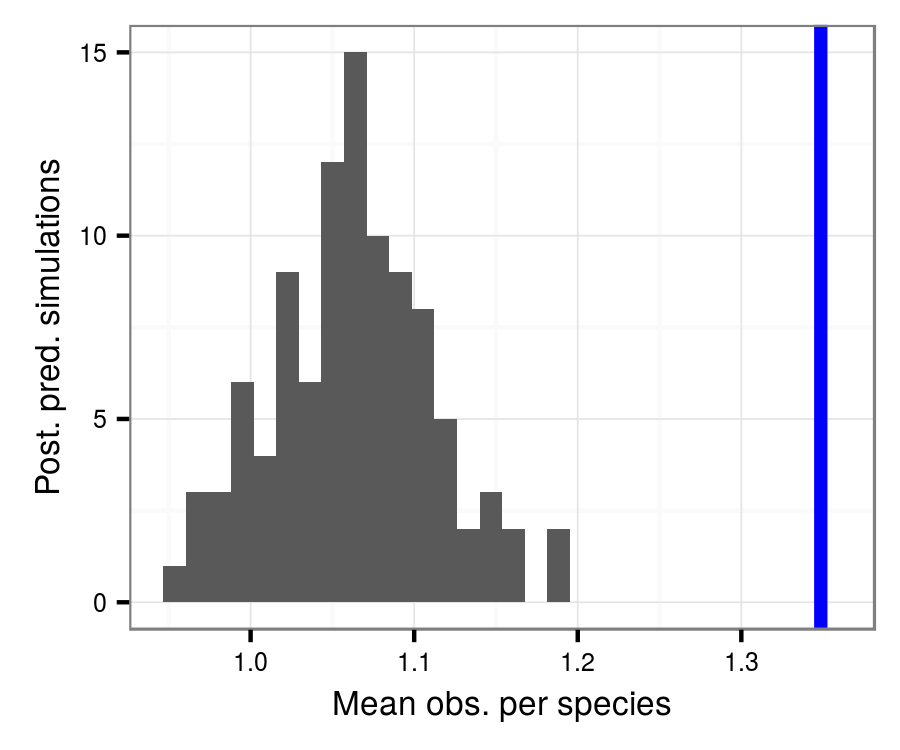
\includegraphics[width=\textwidth,height=0.4\textheight,keepaspectratio=true]{figure/pred_occ}
    \caption{Pure-presence model}
    \label{fig:ppc_pure_presence}
  \end{subfigure}
  \begin{subfigure}[b]{0.45\textwidth}
    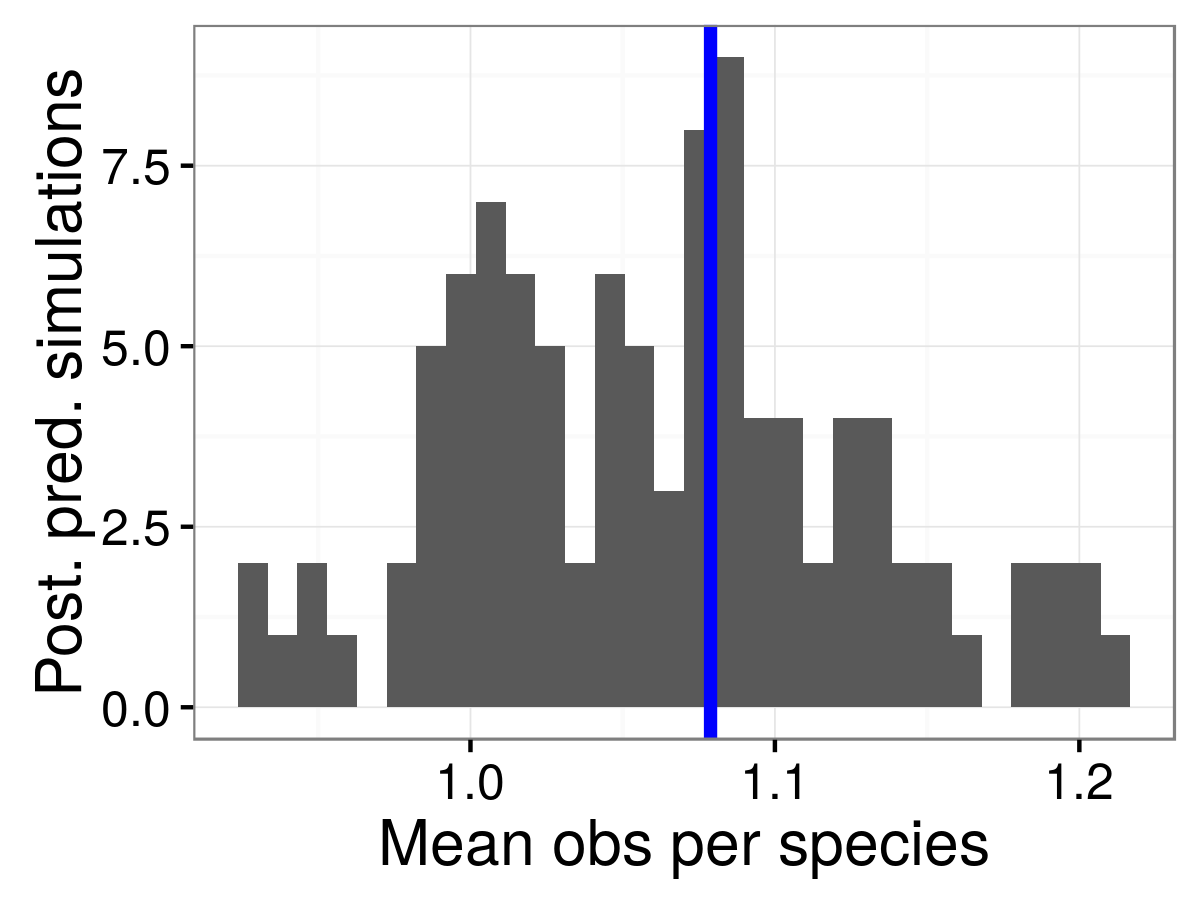
\includegraphics[width=\textwidth,height=0.4\textheight,keepaspectratio=true]{figure/pred_occ_bd}
    \caption{Birth-death model}
    \label{fig:ppc_birth_death}
  \end{subfigure}
  \caption[Posterior predictive check of average occurrence]{Comparison of the average observed number of occurrences per species (blue line) to the average number of occurrences from 100 posterior predictive datasets using the posterior estimates from the pure-presence and birth-death models.}
\end{figure}


% need to inspect the posterior estimates in order to understand the differences
%   ecotype occurrence (pp), origination + survival (bd) probabilities
%   effect of mass on 
%     preservation (pp, bd)
%     occurrence (pp)
%     origination + survival (bd)
%   group-level covariates on 
%     occurrence (pp)
%     origination + survival (bd)

Occurrence probabilities estimated from the pure-presence model (Fig. \ref{fig:eco_occur}) are much more similar to the origination estimates from the birth-death model (Fig. \ref{fig:eco_origin}) than the estimates of survival probability (Fig. \ref{fig:eco_survival}). 

In general, both occurrence probabilities estimated from the pure-presence model (Fig. \ref{fig:eco_occur}) and origination probabilities estimated from the birth-death model (fig. \ref{fig:eco_origin}) increase with time. Notable, ecotypes with arboreal components do not follow this average; instead, occurrence and origination probabilities appear relatively flat for most of the Cenozoic.

The dramatic differences between origination and survival probabilities indicate how different these processes are, and may be responsible for the better posterior predictive perfomance of the birth-death model over the pure-presence model (Fig. \ref{fig:ppc_pure_presence}, and \ref{fig:ppc_birth_death}). While the estimates of both time series have high variance, what is striking is how mean origination probability changes over time while in general survival probabilities have relatively stable means (Fig. \ref{fig:eco_origin}, and \ref{fig:eco_survival}).

Estimates of origination probabilities appear to have less uncertainty than for survival (Fig. \ref{fig:eco_origin}, and \ref{fig:eco_survival}).


\begin{figure}[ht]
  \centering
  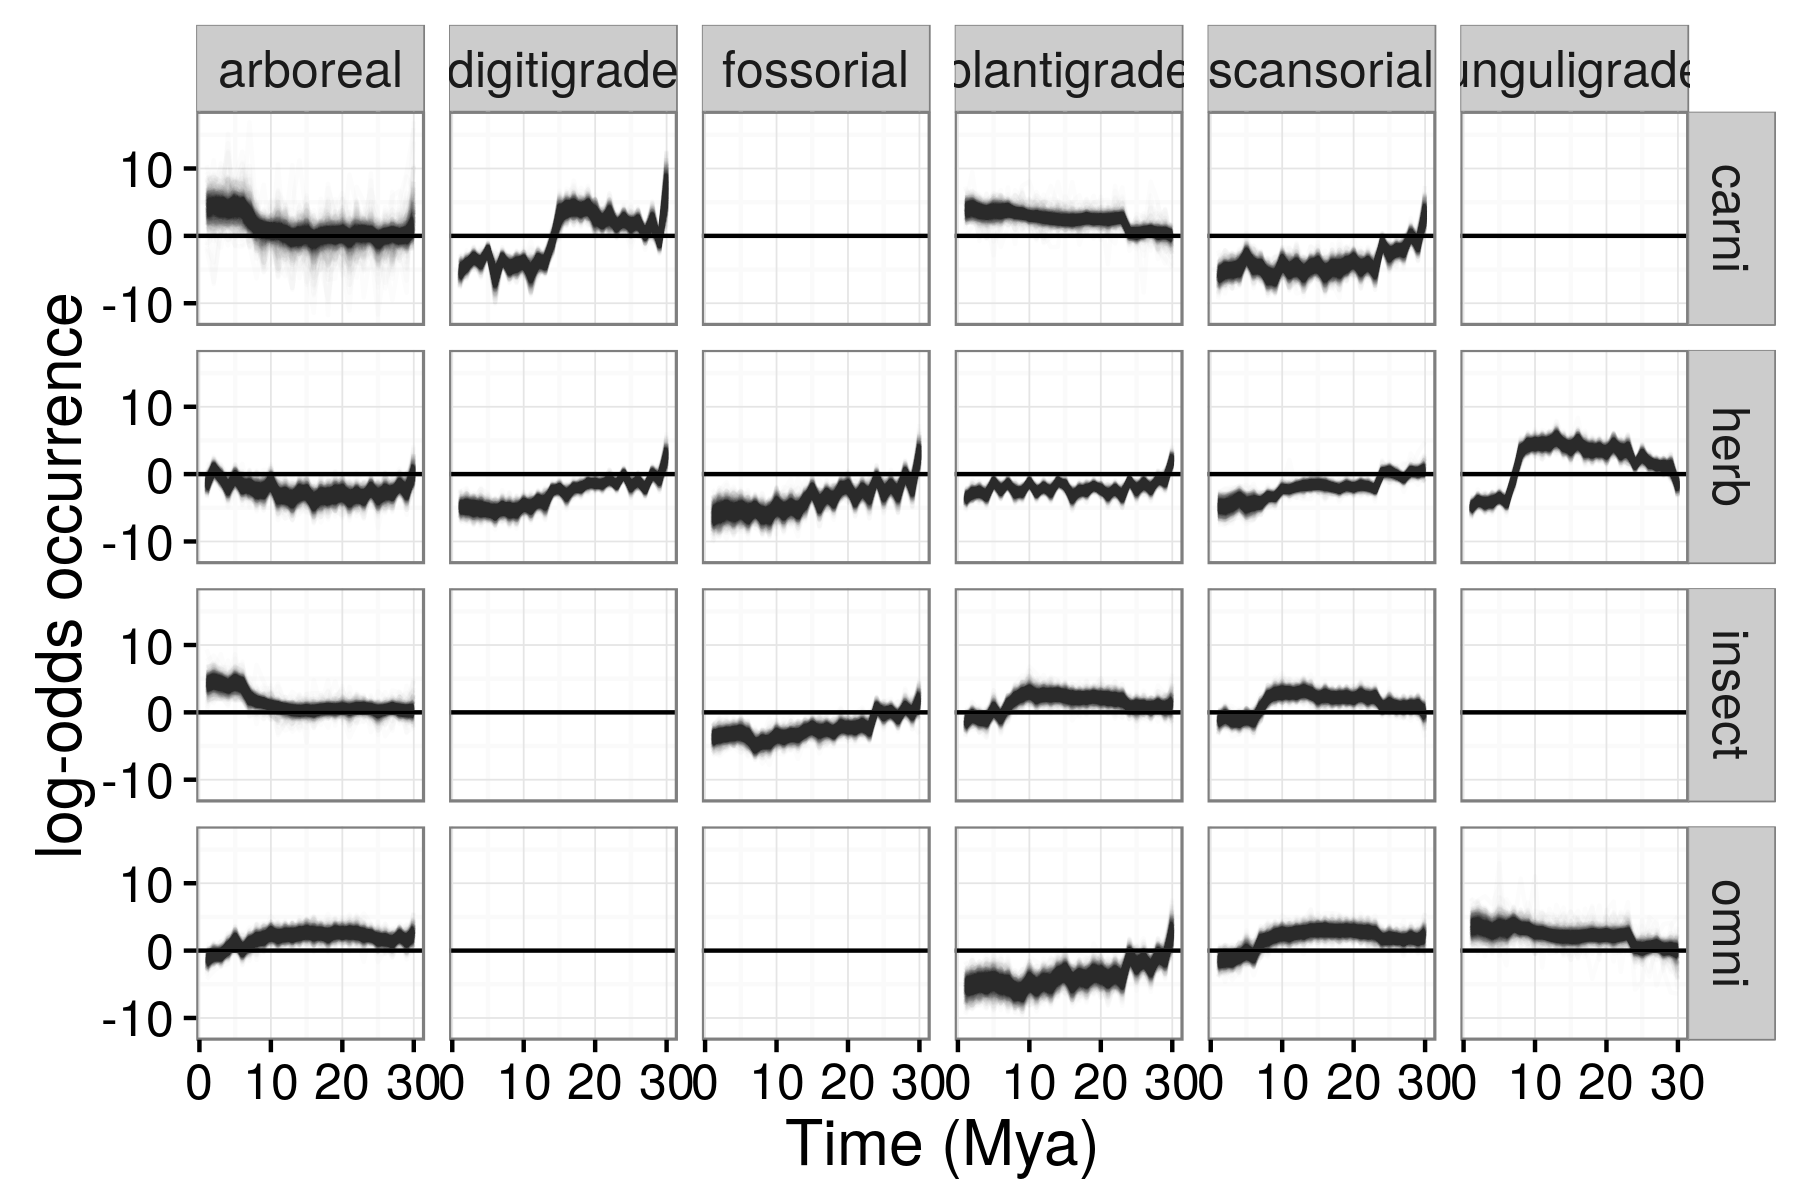
\includegraphics[width=\textwidth,height=0.8\textheight,keepaspectratio=true]{figure/ecotype_occurrence}
  \caption[Ecotype occurrence probability estimated from the pure-presence model]{Probability of a mammal ecotype occurring over time as estimated from the pure-presence model. Each panel depicts 100 random samples from the model's posterior. The columns are by locomotor category and rows by dietary category; their intersections are the observed and analyzed ecotypes. Panels with no lines are ecotypes not observed in the dataset.}
  \label{fig:eco_occur}
\end{figure}

\begin{figure}[ht]
  \centering
  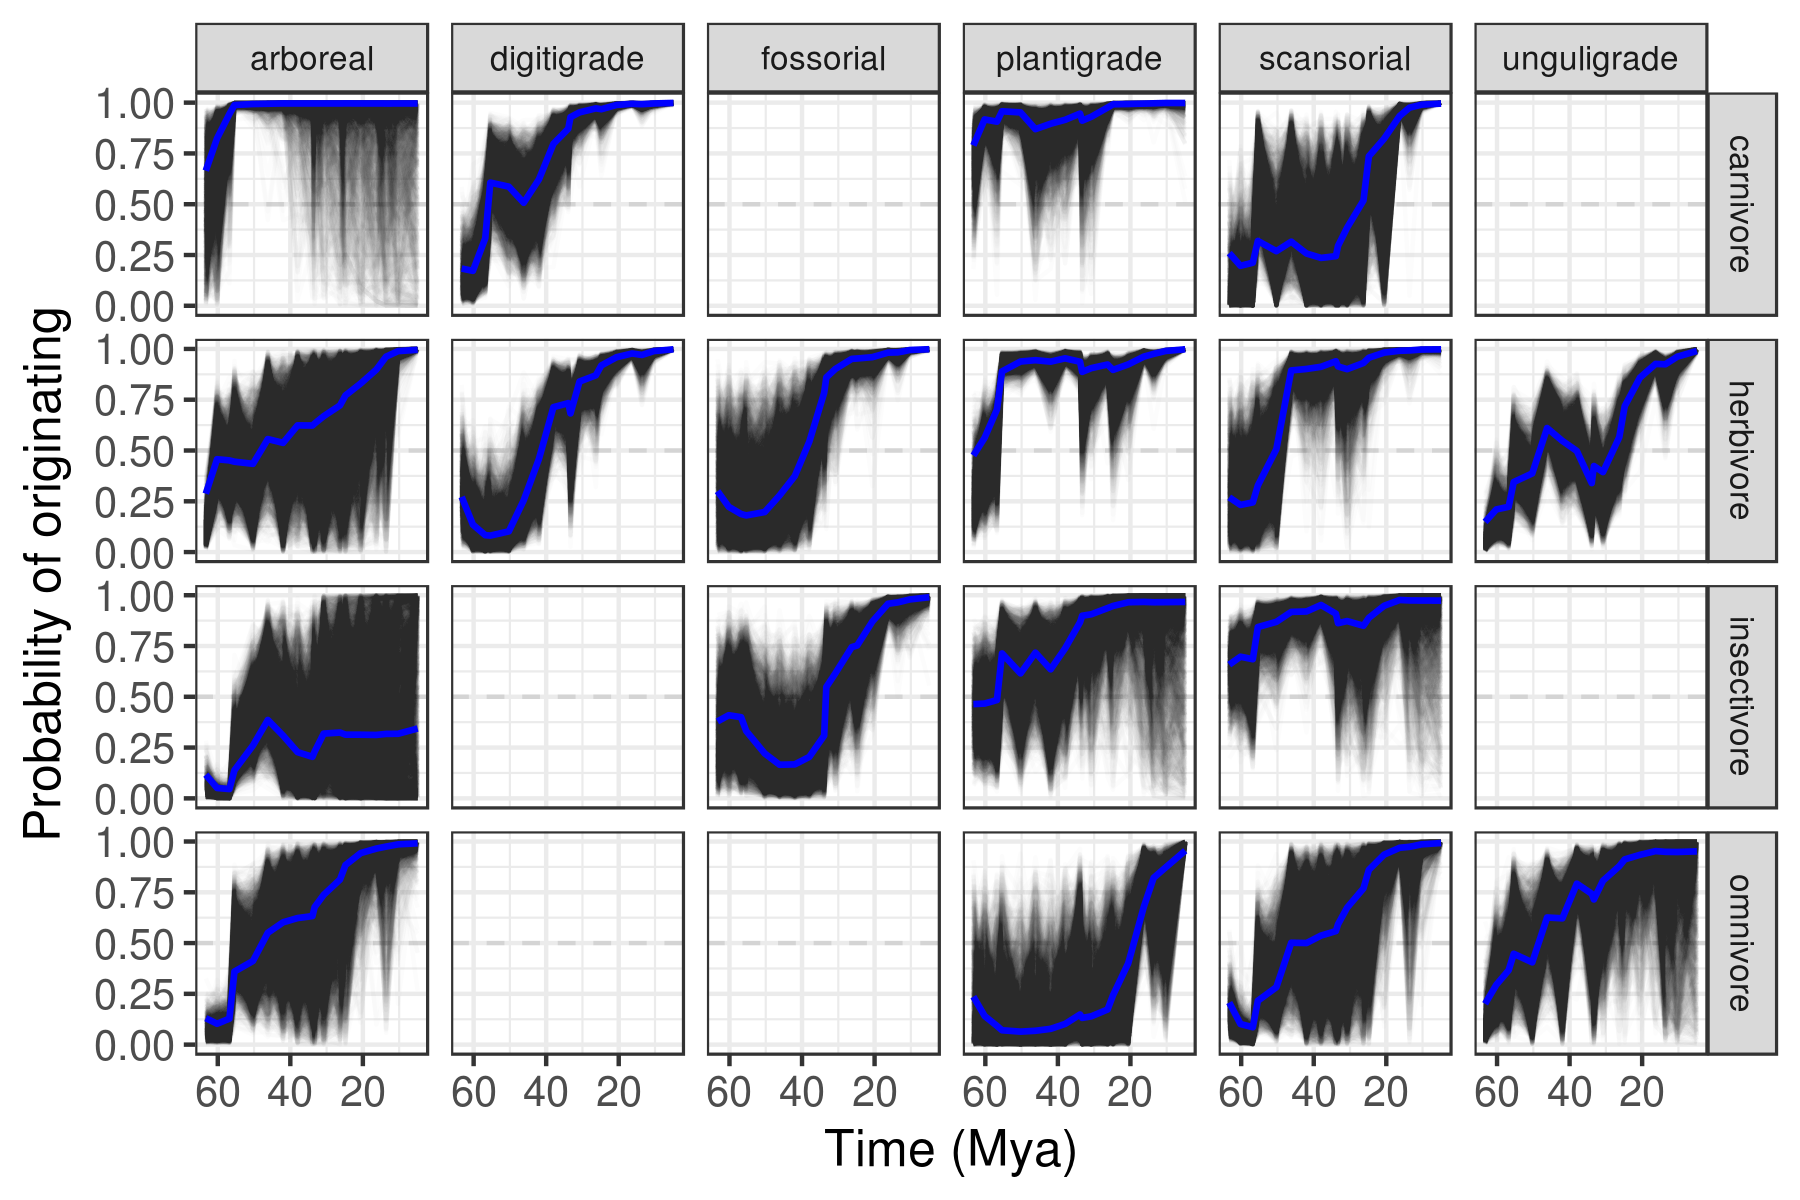
\includegraphics[width=\textwidth,height=0.8\textheight,keepaspectratio=true]{figure/ecotype_origin_bd}
  \caption[Ecotype origination probability estimated from the birth-death model]{Probability of a mammal ecotype origination probabliities at each time point as estimated from the birth-death model. Each panel depicts 100 random samples from the model's posterior. The columns are by locomotor category and rows by dietary category; their intersections are the observed and analyzed ecotypes. Panels with no lines are ecotypes not observed in the dataset.}
  \label{fig:eco_origin}
\end{figure}

\begin{figure}[ht]
  \centering
  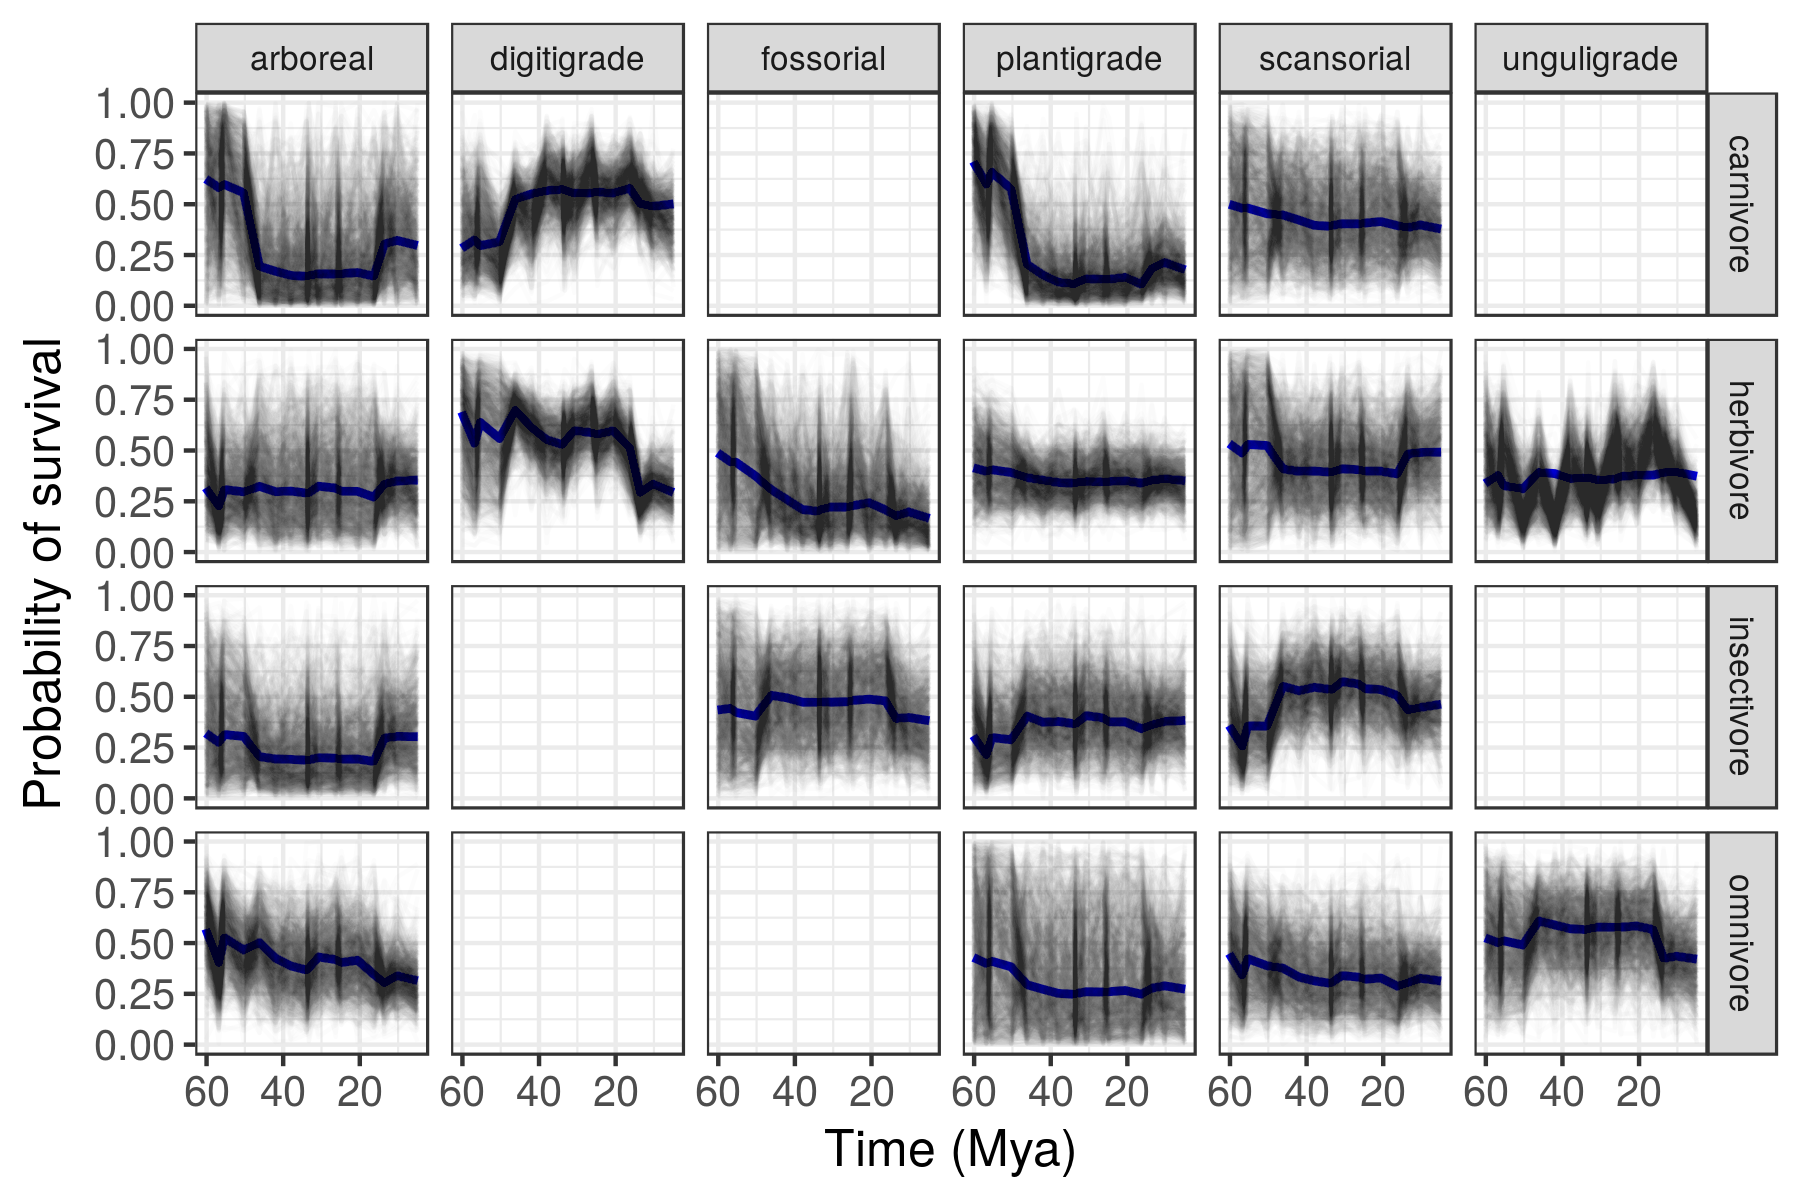
\includegraphics[width=\textwidth,height=0.8\textheight,keepaspectratio=true]{figure/ecotype_survival_bd}
  \caption[Ecotype survival probability estimated from the birth-death model]{Probability of a mammal ecotype survival probabilities at each time point as estimated from the birth-death model. Each panel depicts 100 random samples from the model's posterior. The columns are by locomotor category and rows by dietary category; their intersections are the observed and analyzed ecotypes. Panels with no lines are ecotypes not observed in the dataset.}
  \label{fig:eco_survival}
\end{figure}





The pure-presence and birth-death models different in estimated effect of mass on the probability of observing a species that is present (Fig. \ref{fig:mass_preserve}). For the pure-presence model, mass is estimated to have no effect on the probability of observing a species that is presence (Fig. \ref{fig:mass_preserve_pure_pres}). Contrastingly, for the birth-death model mass is found to have a negative relationship with observation such that larger species are less likely to be observed if present than smaller species (Fig. \ref{fig:mass_preserve_bd}). 

The result from the birth-death model is unexpected given that it is generally assumed that larger mammals are more likely to have been collected than smaller mammals CITATION. However, collection is not preservation; similarities in preservation rate indicate similarities in how gap-filled species records are. What this result means is that the record of large bodied species is expected on average to be more gap-filled and less consistent from time point to time point than smaller bodied species. Additionally, this is presence/absence data, so higher preservation and collection in terms of individual specimens at a location or a single temporal horizon does not necessarily translate to high preservation over time.


\begin{figure}[ht]
  \begin{subfigure}[b]{0.45\textwidth}
    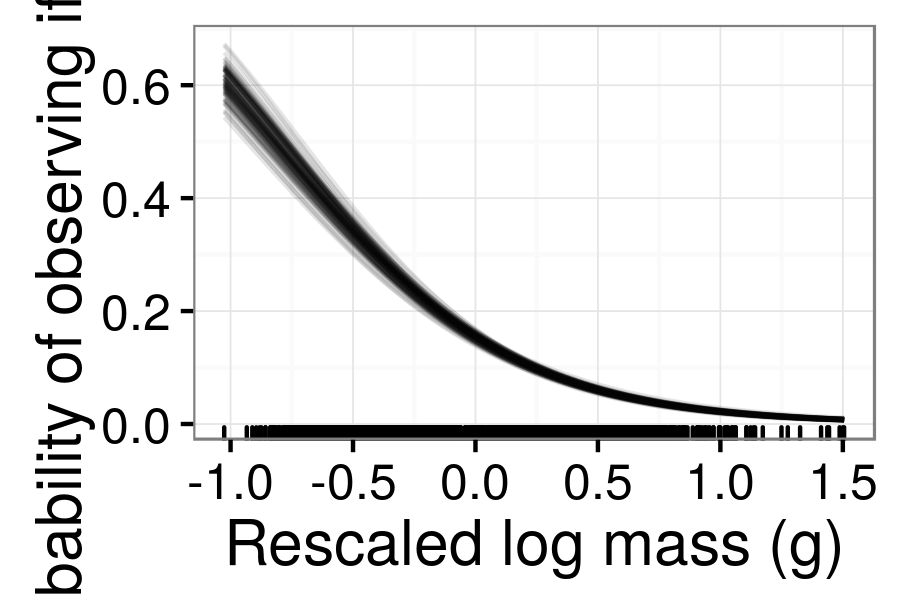
\includegraphics[width=\textwidth,height=0.8\textheight,keepaspectratio=true]{figure/mass_on_samp}
    \caption{Pure-presence model}
    \label{fig:mass_preserve_pure_pres}
  \end{subfigure}
  \begin{subfigure}[b]{0.45\textwidth}
    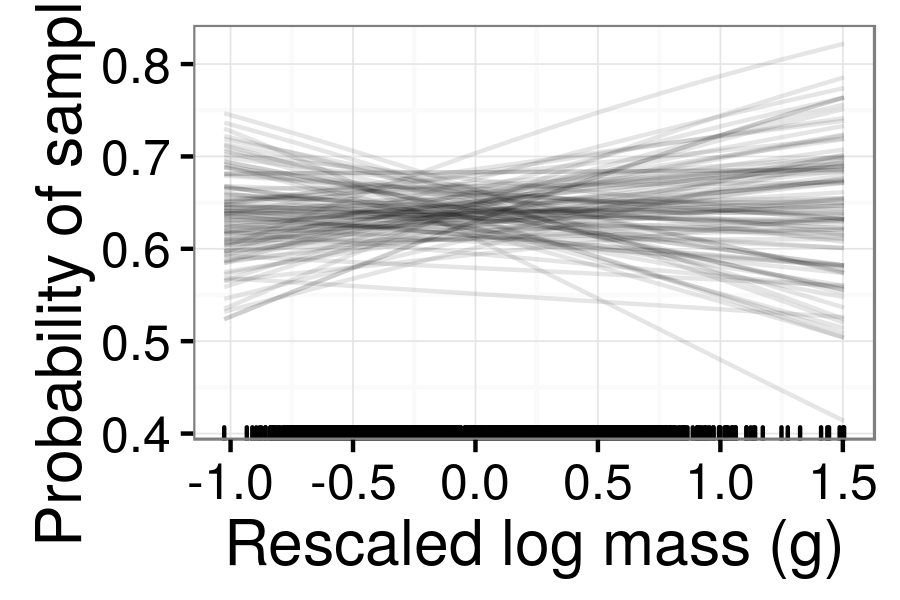
\includegraphics[width=\textwidth,height=0.8\textheight,keepaspectratio=true]{figure/mass_on_samp_bd}
    \caption{Birth-death model}
    \label{fig:mass_preserve_bd}
  \end{subfigure}
  \caption[Estimates of the effect of mass on observation probability]{Estimates of the effect of species mass on probability of observing a present species (\(p\)). Mass has been log-transformed, centered, and rescaled; this means that a mass of 0 corresponds to the mean of log-mass of all observed species and that mass is in standard deviation units. Estimates are from both the pure-presence and birth-death models.}
  \label{fig:mass_preserve}
\end{figure}




The effect of species mass on probability of occurrence as estimated from the pure-presence (Fig. \ref{fig:mass_occur}) is most similar to the effect of species mass on probability of origination as estimates from the birth-death model (Fig. \ref{fig:mass_origin}). The striking pattern observable in both sets of estimates is the higher probability of occurrence for species with body sizes closer to the mean than either extremes. This result is consistent with the canonically normal distribution of mammal body sizes CITATION; it is then expected that the most likely to occur species would be those from the middle of the distribution, and that species originating will on average be of average mass, especially considering species shared common ancestry CITATION.

\begin{figure}[ht]
  \centering
  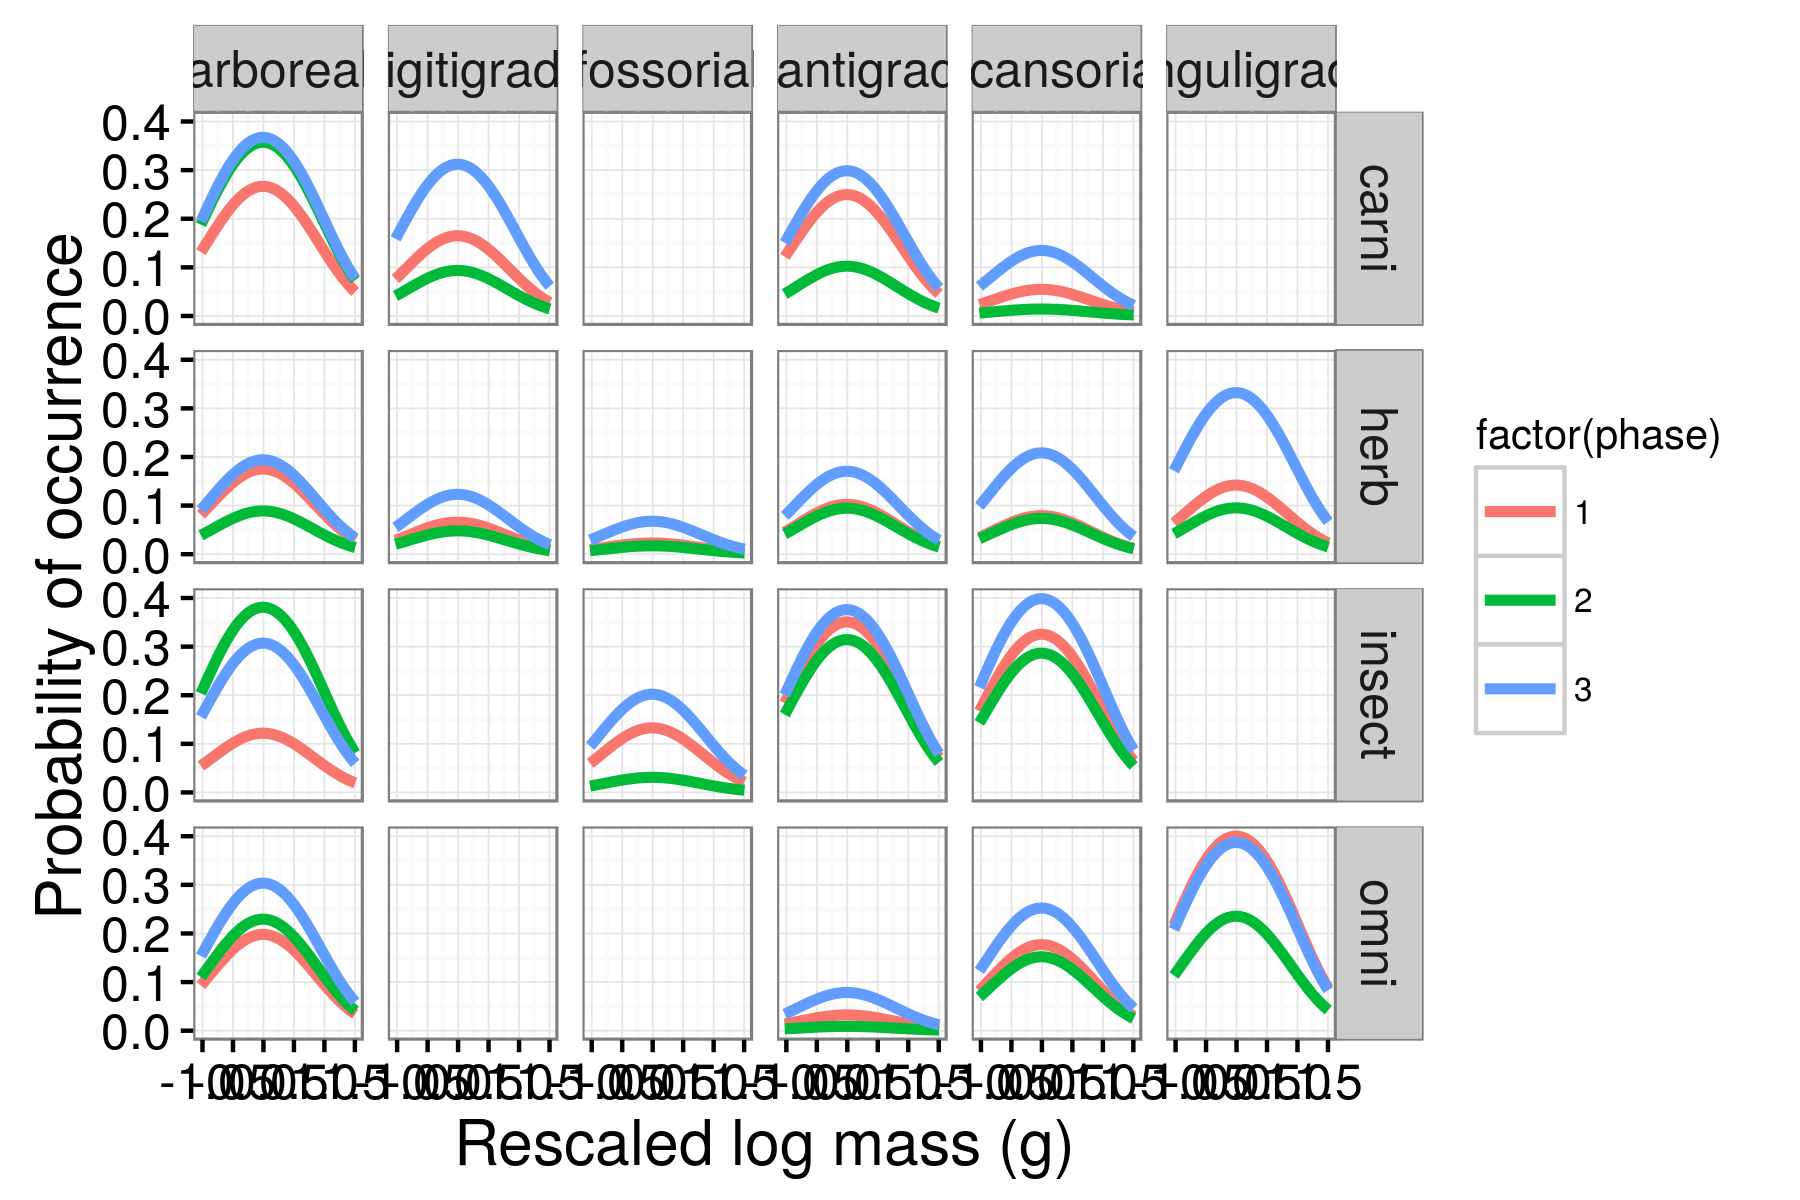
\includegraphics[width=\textwidth,height=0.8\textheight,keepaspectratio=true]{figure/mass_on_pres}
  \caption[Effect of mass on probability of species occurrence as estimated from the pure-presence model]{Mean estimate of the effect of species mass on the probability of a species occurrence for each of the three plant phases. The effect of mass is considered constant over time and that the only aspect of the model that changes with plant phase is the intercept of the relationship between mass and occurrence. The three plant phases are indicated by the color of the line. Mass has been log-transformed, centered, and rescaled; this means that a mass of 0 corresponds to the mean of log-mass of all observed species and that mass is in standard deviation units. Only the mean estimates of the effects of both mass and plant phase are plotted for clarity; these estimates are obviously made with uncertainty.}
  \label{fig:mass_occur}
\end{figure}

\begin{figure}[ht]
  \centering
  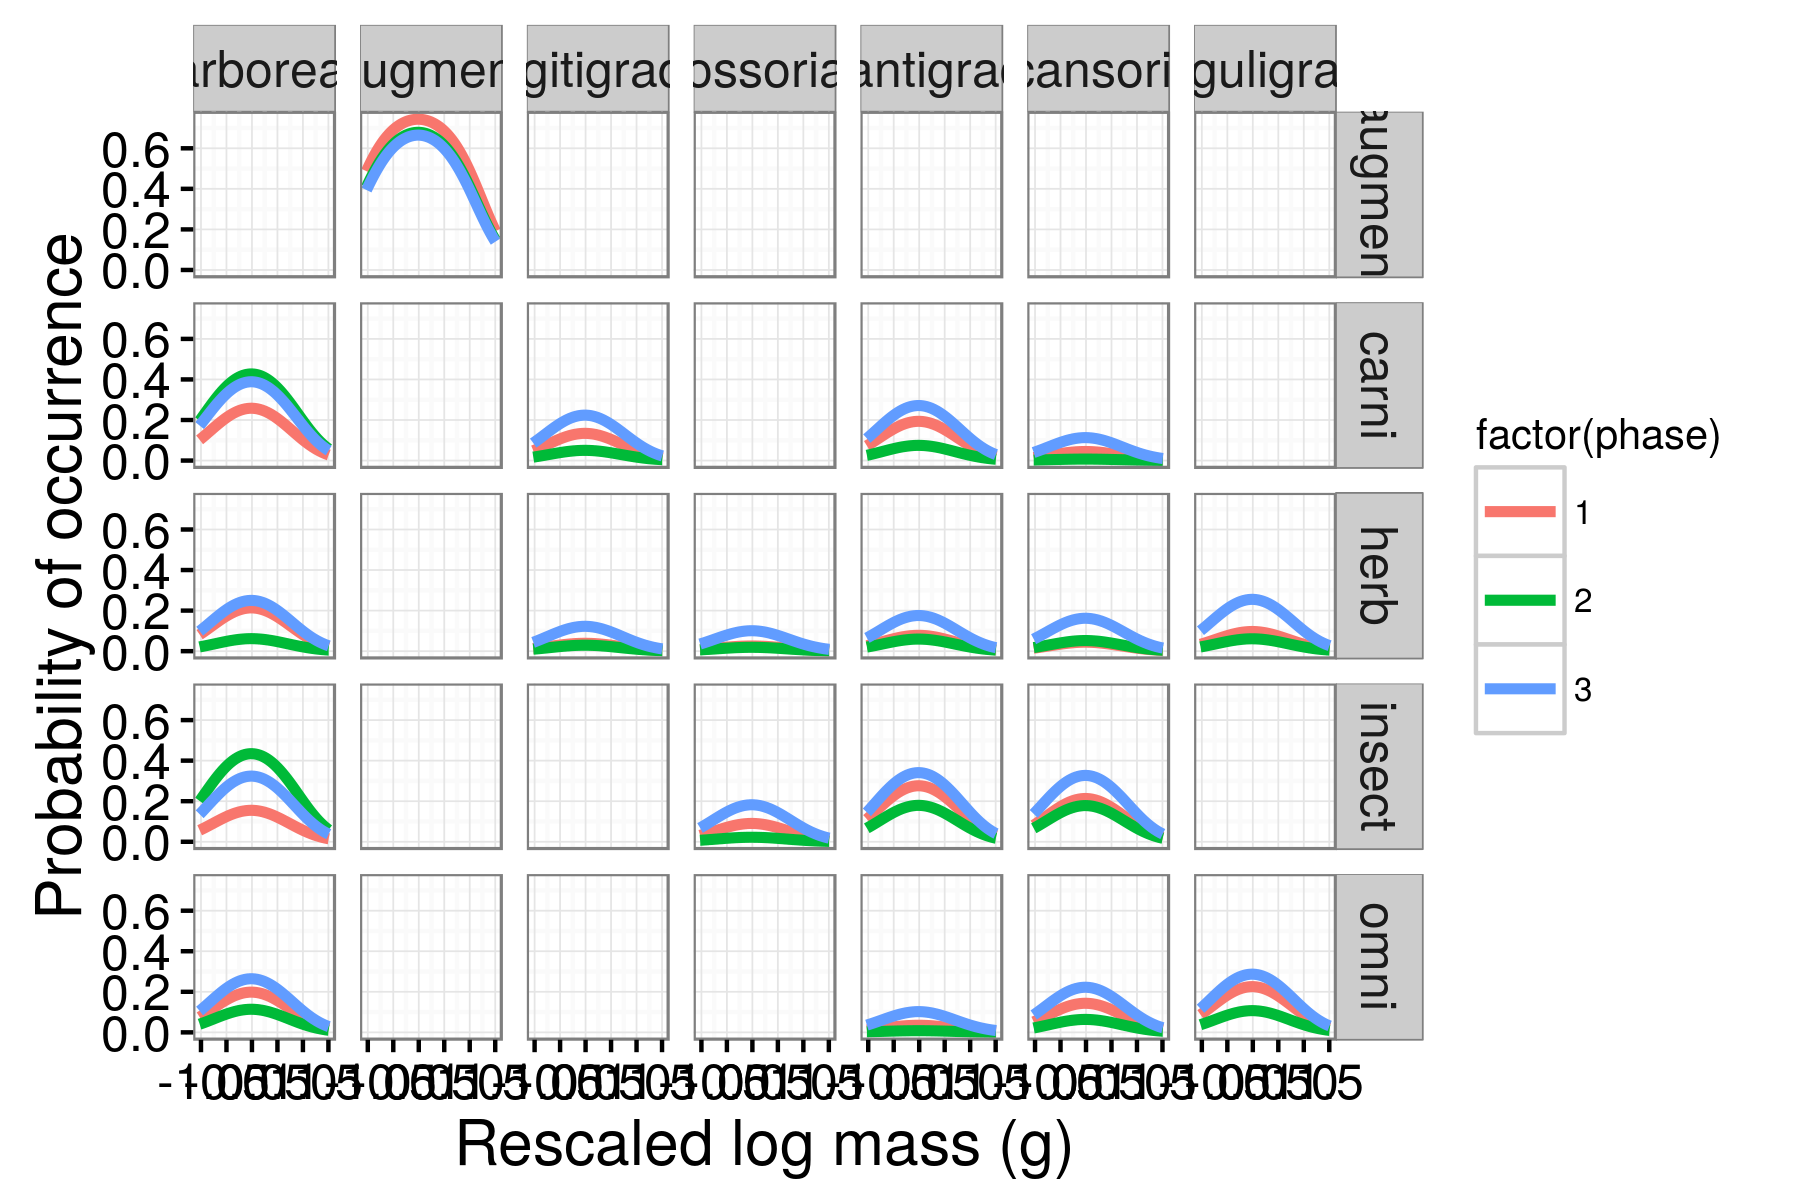
\includegraphics[width=\textwidth,height=0.8\textheight,keepaspectratio=true]{figure/mass_on_origin_bd}
  \caption[Effect of mass on probability of species origination as estimated from the birth-death model]{Mean estimate of the effect of species mass on the probability of a species originating for each of the three plant phases. The effect of mass is considered constant over time and that the only aspect of the model that changes with plant phase is the intercept of the relationship between mass and origination. The three plant phases are indicated by the color of the line. Mass has been log-transformed, centered, and rescaled; this means that a mass of 0 corresponds to the mean of log-mass of all observed species and that mass is in standard deviation units. Only the mean estimates of the effects of both mass and plant phase are plotted for clarity; these estimates are obviously made with uncertainty.}
  \label{fig:mass_origin}
\end{figure}

In contrast, the effect of species mass on probability of survival as estimated from the birth-death model (Fig. \ref{fig:mass_survival}) indicates little effect of mass on extinction; this is consistent with previous findings from the North American mammal fossil record \citep{Smits2015b,Tomiya2013}. Note that all variation between ecotypes is due to differences in ecotype-specific survival probability and the associated effects of plant phase.

\begin{figure}[ht]
  \centering
  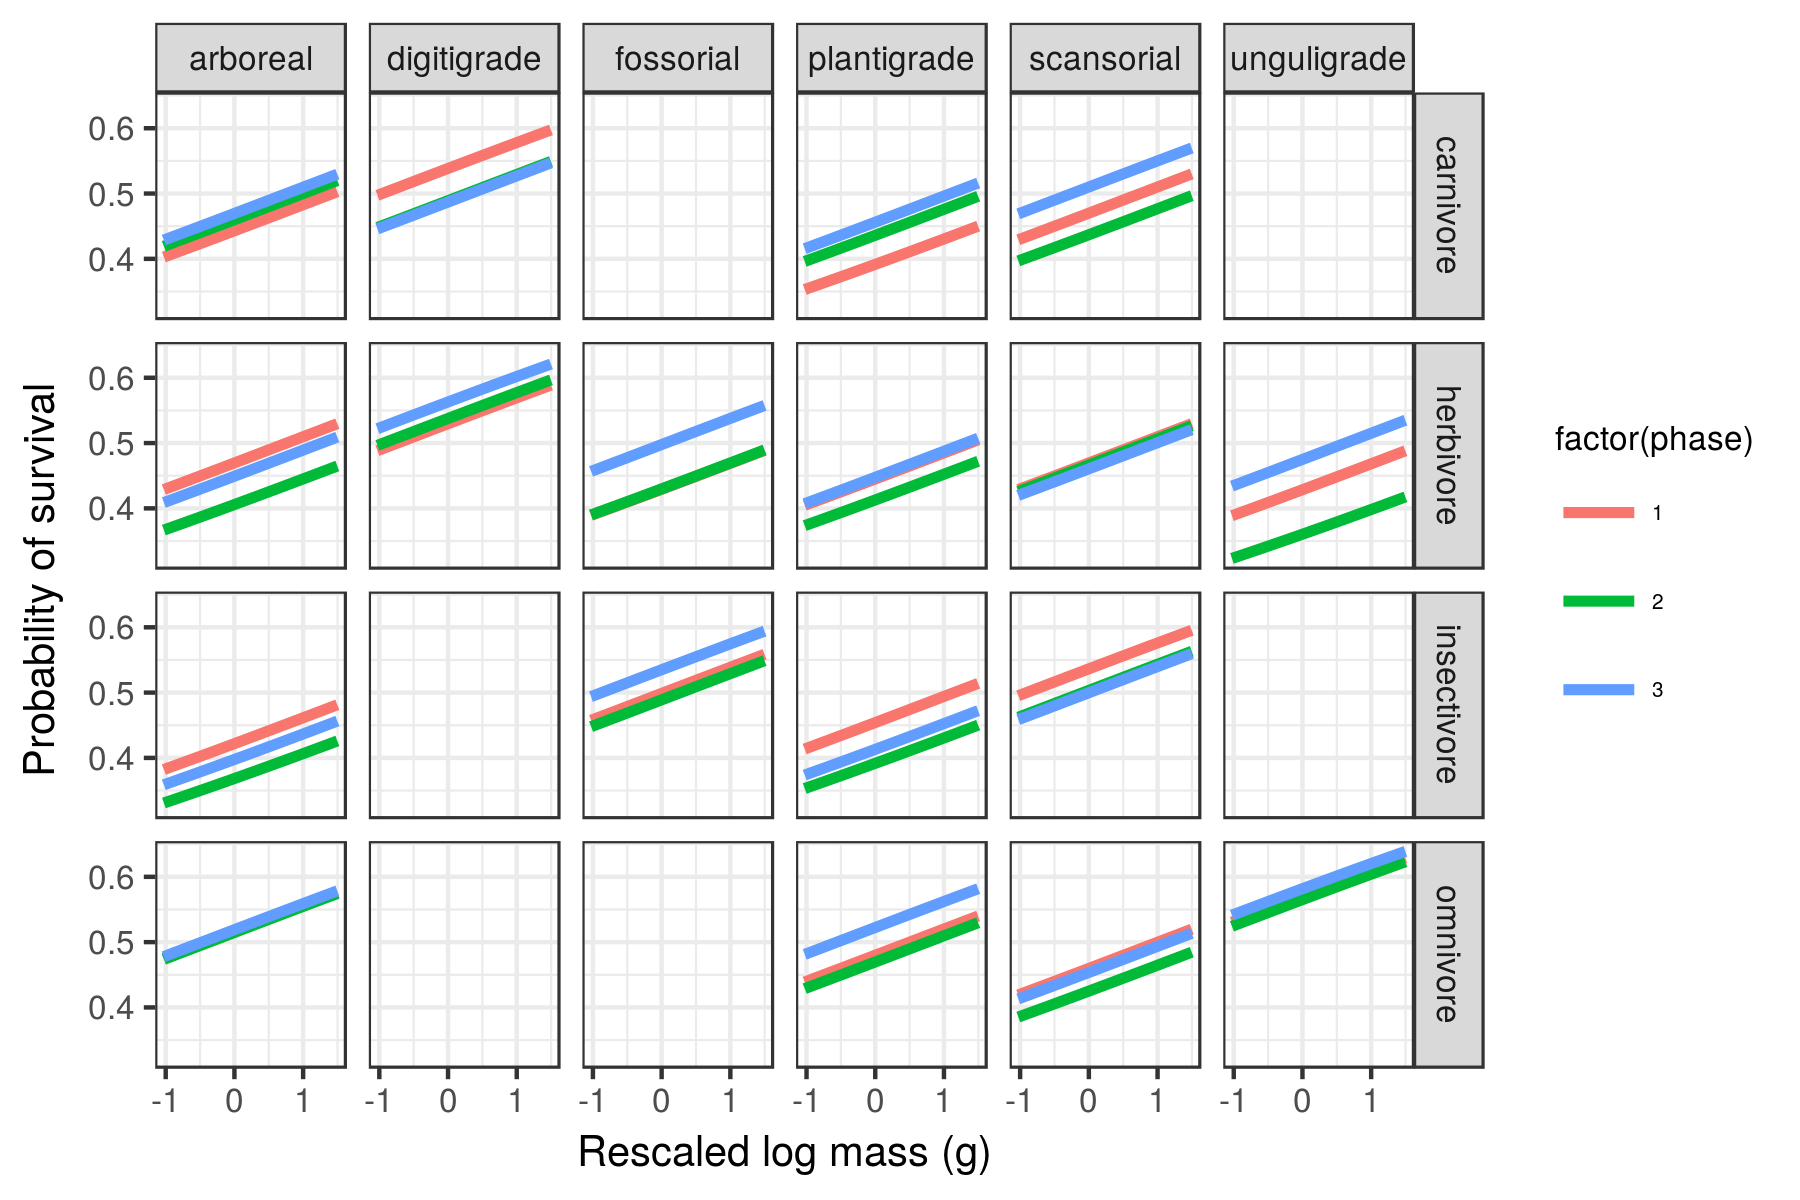
\includegraphics[width=\textwidth,height=0.8\textheight,keepaspectratio=true]{figure/mass_on_surv_bd}
  \caption[Effect of mass on probability of species survival as estimated from the birth-death model]{Mean estimate of the effect of species mass on the probability of a species survival for each of the three plant phases. The effect of mass is considered constant over time and that the only aspect of the model that changes with plant phase is the intercept of the relationship between mass and survival. The three plant phases are indicated by the color of the line. Mass has been log-transformed, centered, and rescaled; this means that a mass of 0 corresponds to the mean of log-mass of all observed species and that mass is in standard deviation units. Only the mean estimates of the effects of both mass and plant plant are plotted for clarity; these estimates are obviously made with uncertainty.}
  \label{fig:mass_survival}
\end{figure}



Similarities in parameters estimates between ecotypes may be due to similar response to environmental factors. Some of the obvious patterns from inspection of the individual-level estimates of occurrence (Fig. \ref{fig:eco_occur}), origination (Fig. \ref{fig:eco_origin}), and survival probabilities (Fig. \ref{fig:eco_survival}) that are of note are the similarities between arboreal taxa and the differences between arboreal and all other taxa.

Inspection of parameter estimates for the group-level covariates 


\begin{figure}[ht]
  \centering
  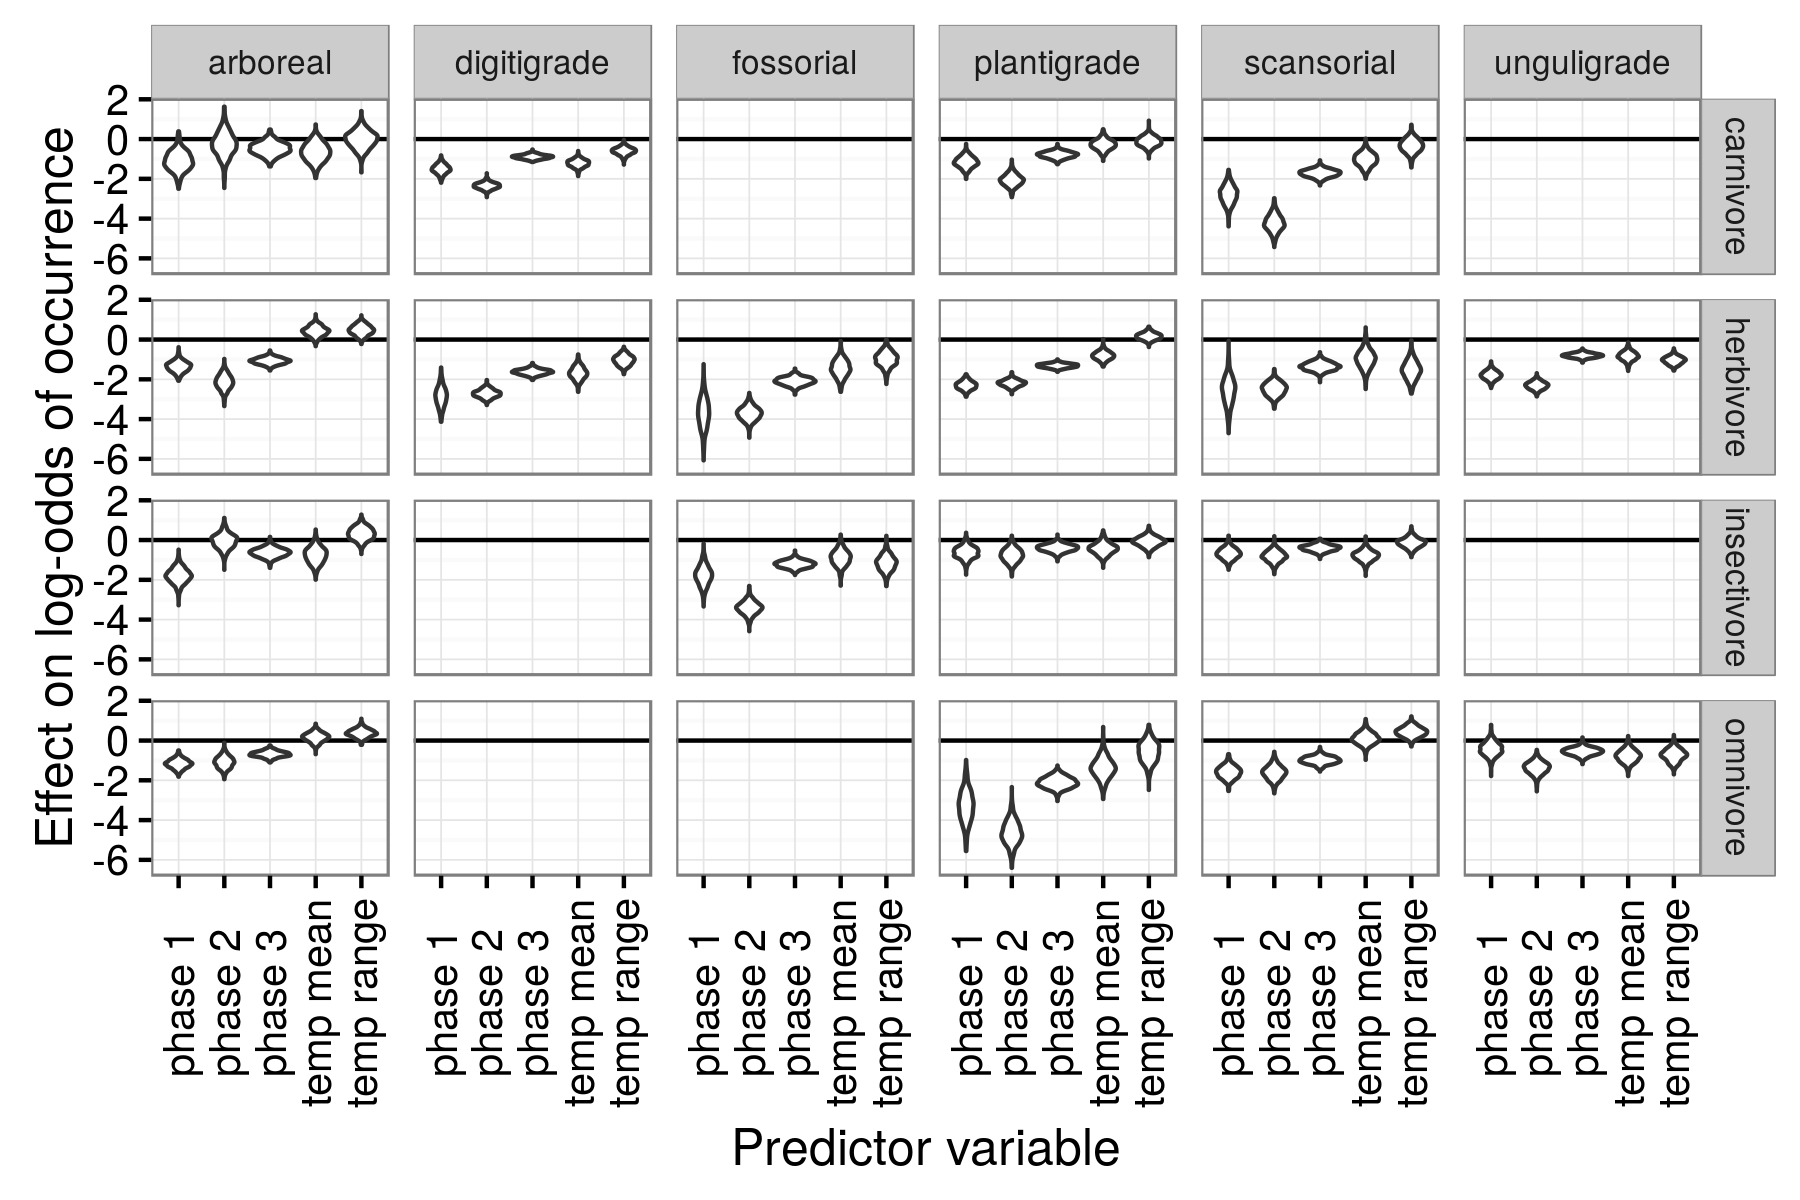
\includegraphics[width=\textwidth,height=0.8\textheight,keepaspectratio=true]{figure/group_on_ecotype}
  \caption[Effects of group-level covariates on log-odds of ecotype occurrence as estimated from the the pure-presence model]{Estimated effects of the group-level covariates describing environmental context on log-odds of species occurrence. These estimates are from the pure-presence model.} 
  \label{fig:group_pure_presence}
\end{figure}

\begin{figure}[ht]
  \centering
  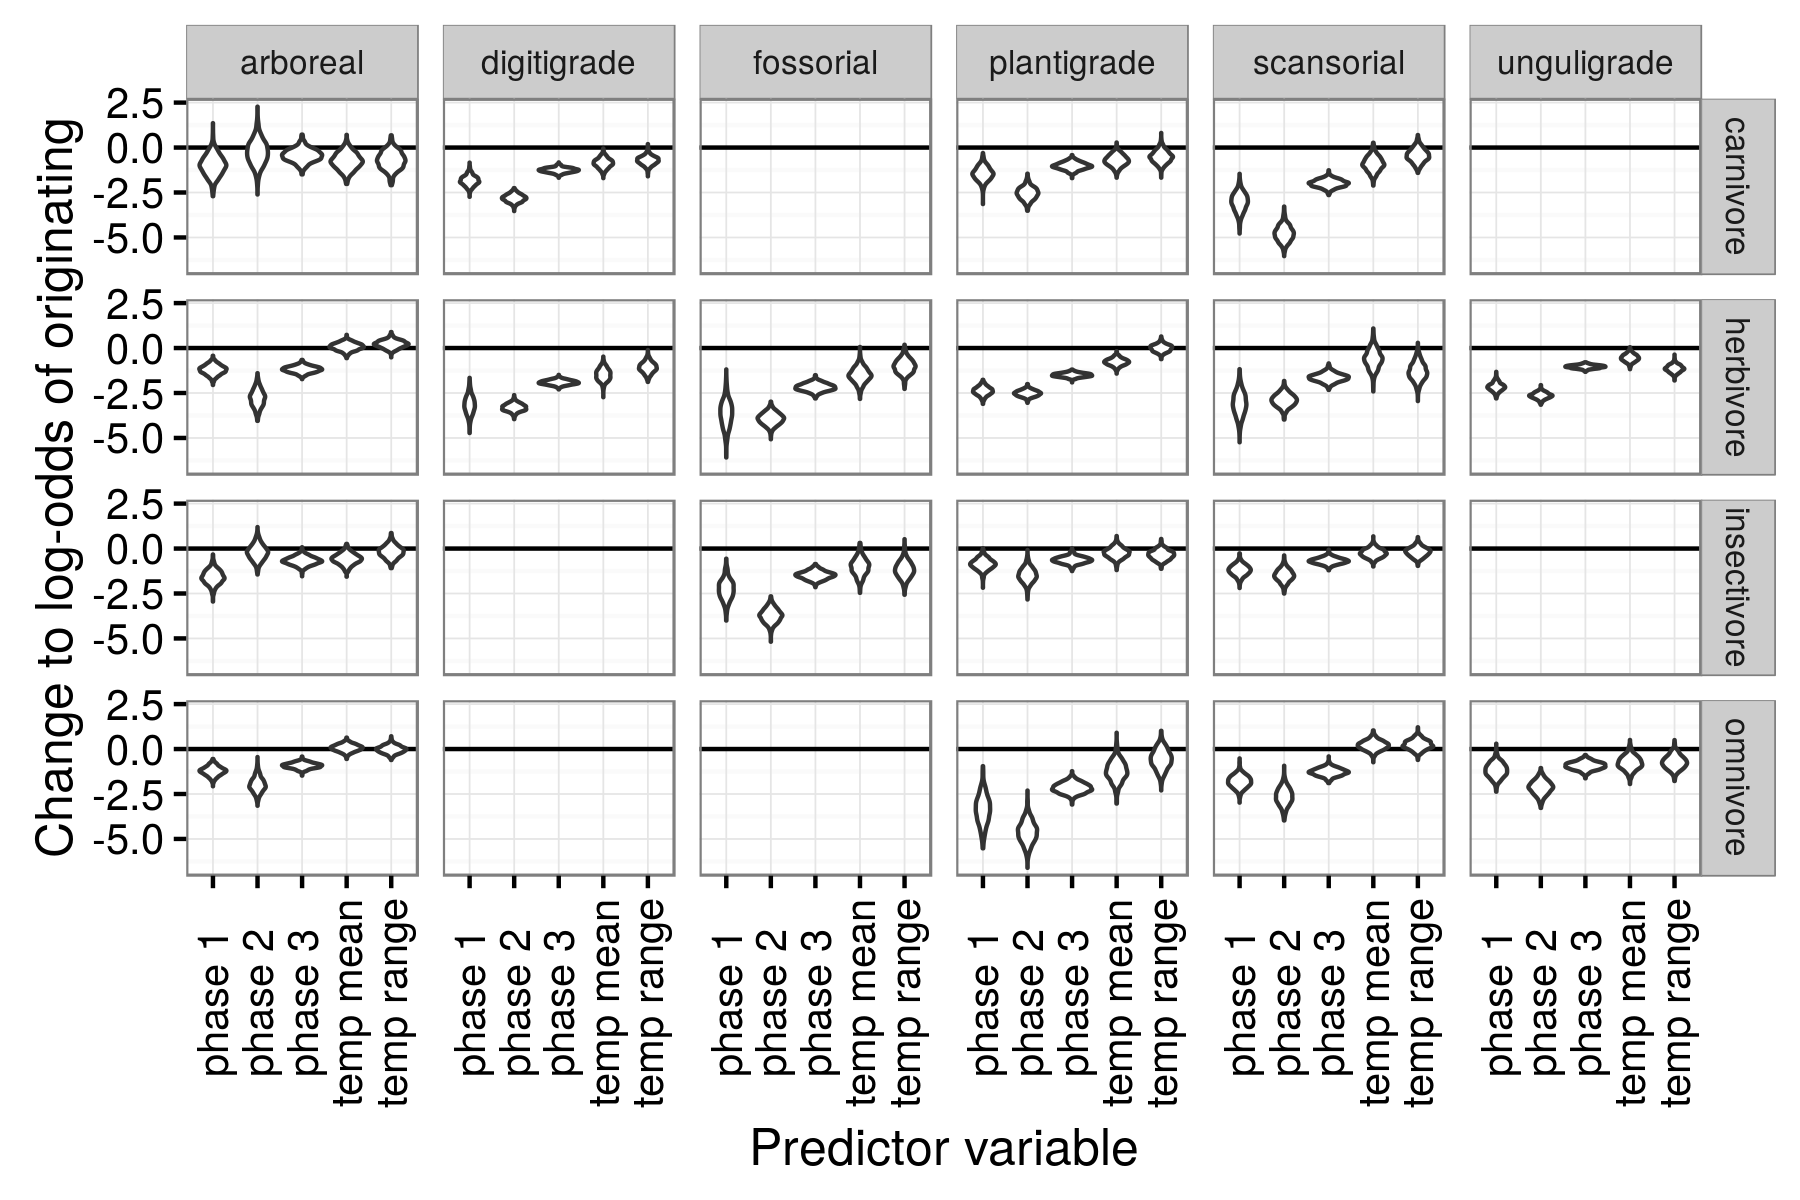
\includegraphics[width=\textwidth,height=0.8\textheight,keepaspectratio=true]{figure/group_on_origin_bd}
  \caption[Effects of group-level covariates on log-odds of ecotype origination as estimated from the the birth-death model]{Estimated effects of the group-level covariates describing environmental context on log-odds of species origination. These estimates are from the birth-death model.}
  \label{fig:group_origin_bd}
\end{figure}

\begin{figure}[ht]
  \centering
  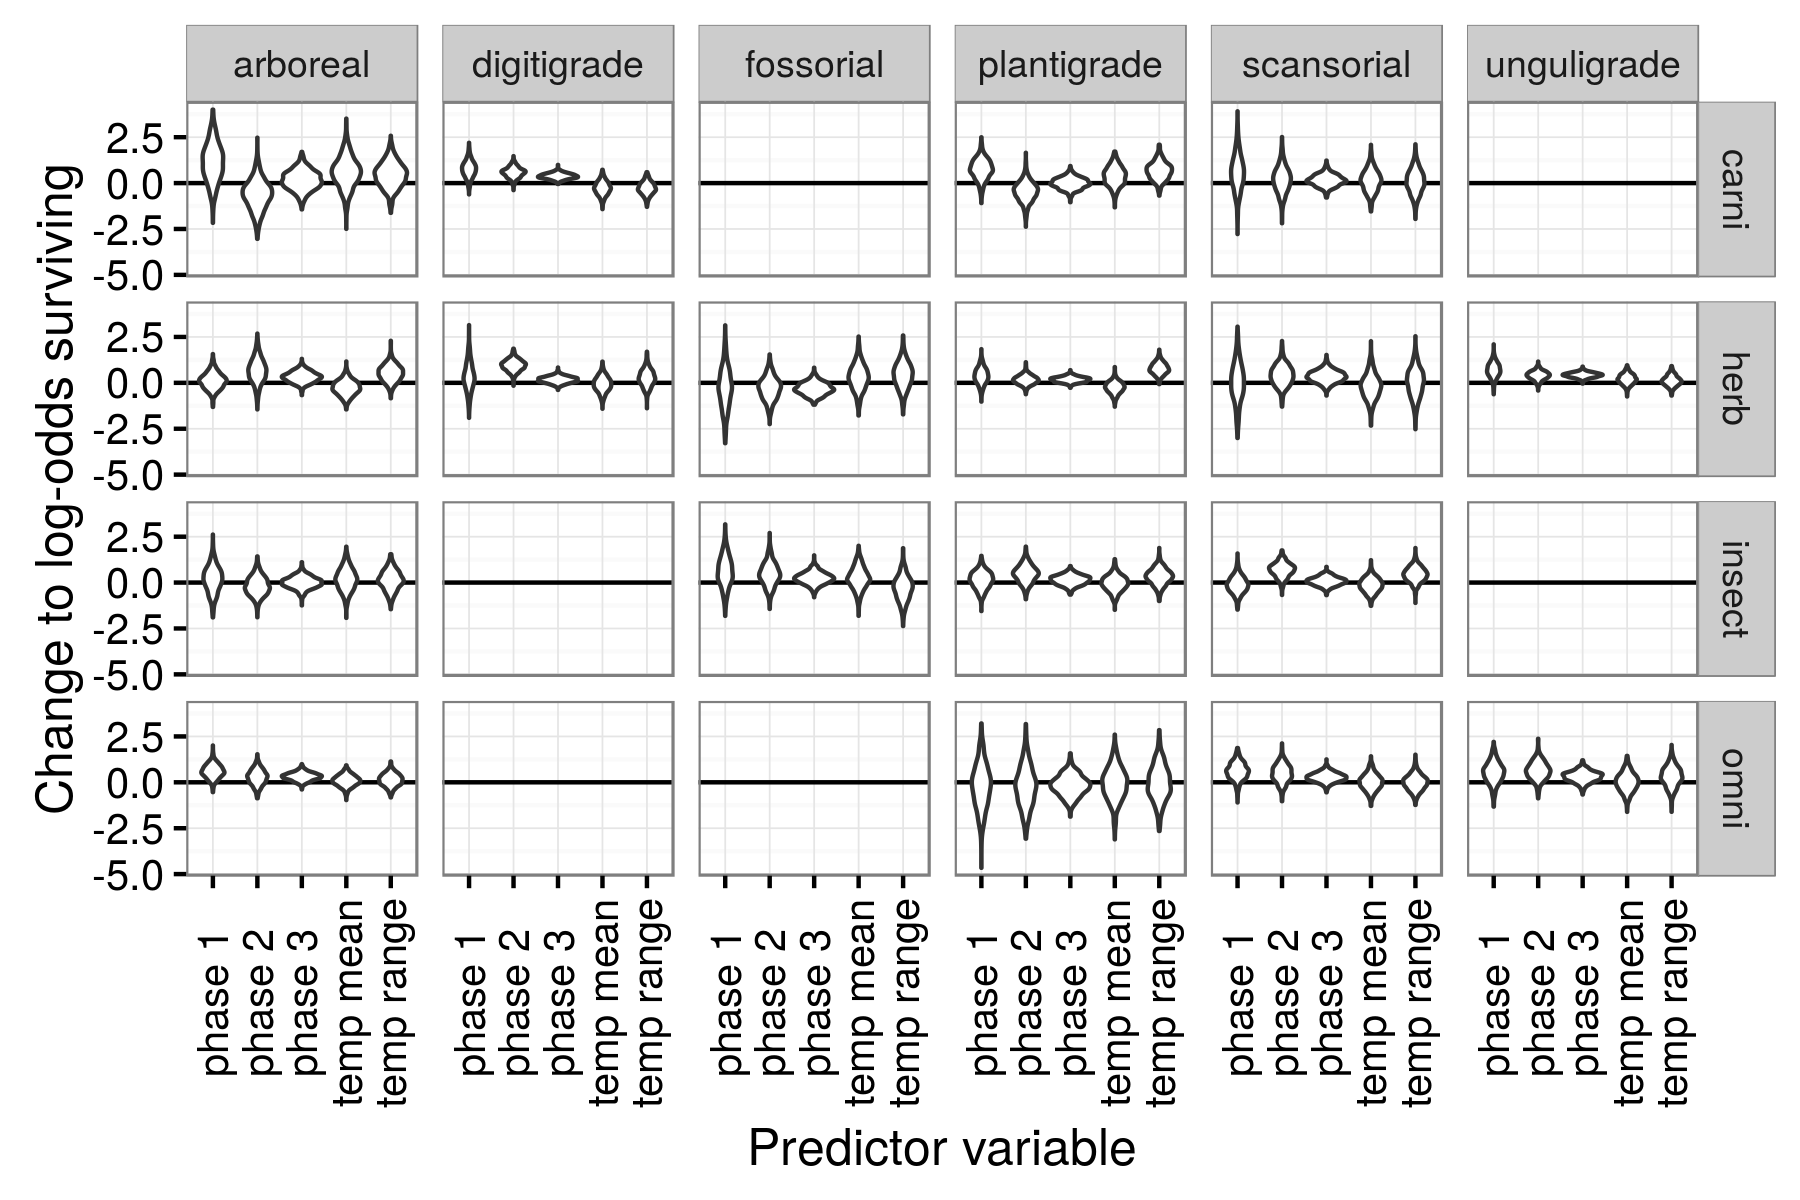
\includegraphics[width=\textwidth,height=0.8\textheight,keepaspectratio=true]{figure/group_on_survival_bd}
  \caption[Effects of group-level covariates on log-odds of ecotype survival as estimated from the the birth-death model]{Estimated effects of the group-level covariates describing environmental context on log-odds of species survlval. These estimates are from the birth-death model.}
  \label{fig:group_surv_bd}
\end{figure}





\subsection*{Analysis of diversity}

All analyses of diversification and macroevolutionary rates has been done using only the birth-death model; this is because of the models better posterior predictive check performance (Fig. \ref{fig:ppc_pure_presence}, and \ref{fig:ppc_birth_death}). 

\begin{figure}[ht]
  \begin{subfigure}[b]{0.45\textwidth}
    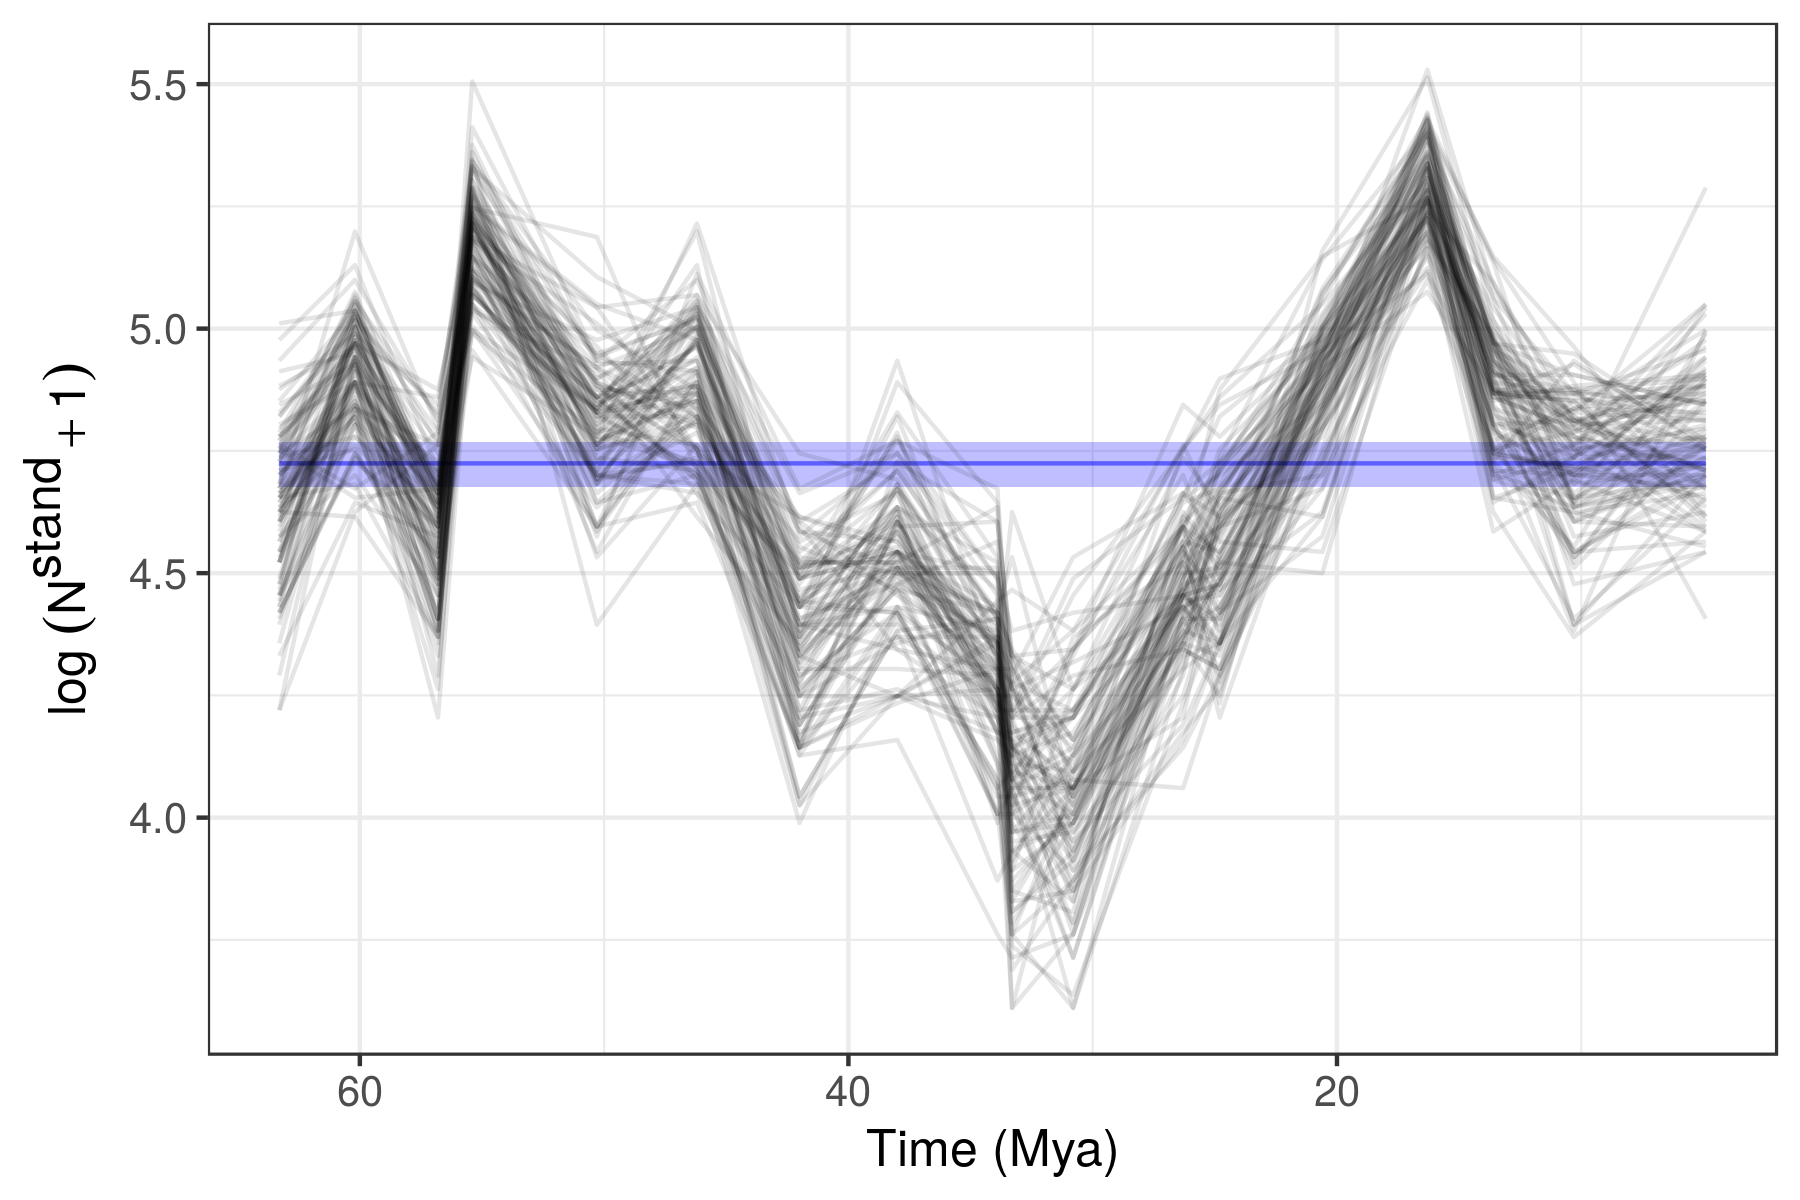
\includegraphics[width=\textwidth,height=0.8\textheight,keepaspectratio=true]{figure/log_diversity}
    \caption{Log diversity}
    %\caption[Estimated mammal log-diversity for the Cenozoic]{Posterior of standing log-diversity of North American mammals for the Cenozoic as estimated from the birth-death model; 100 posterior draws are plotted to indicate the uncertainty in these estimates and what is technically plotted is log of diversity plus 1. The dramatic differences between diversity estimates at the first and second time points and the penultimate and last time points in this series are caused by well known edge effects in discrete-time birth-death models caused by \(p_{\_, t = 1}\) and \(p_{\_, t = T}\) being partially unidentifiable \citep{Royle2008}; the hierarchical modeling strategy used here helps mitigate these effects but they are still present \citep{Gelman2013d,Royle2008}.}
    \label{fig:diversity_est}
  \end{subfigure}
  \begin{subfigure}[b]{0.45\textwidth}
    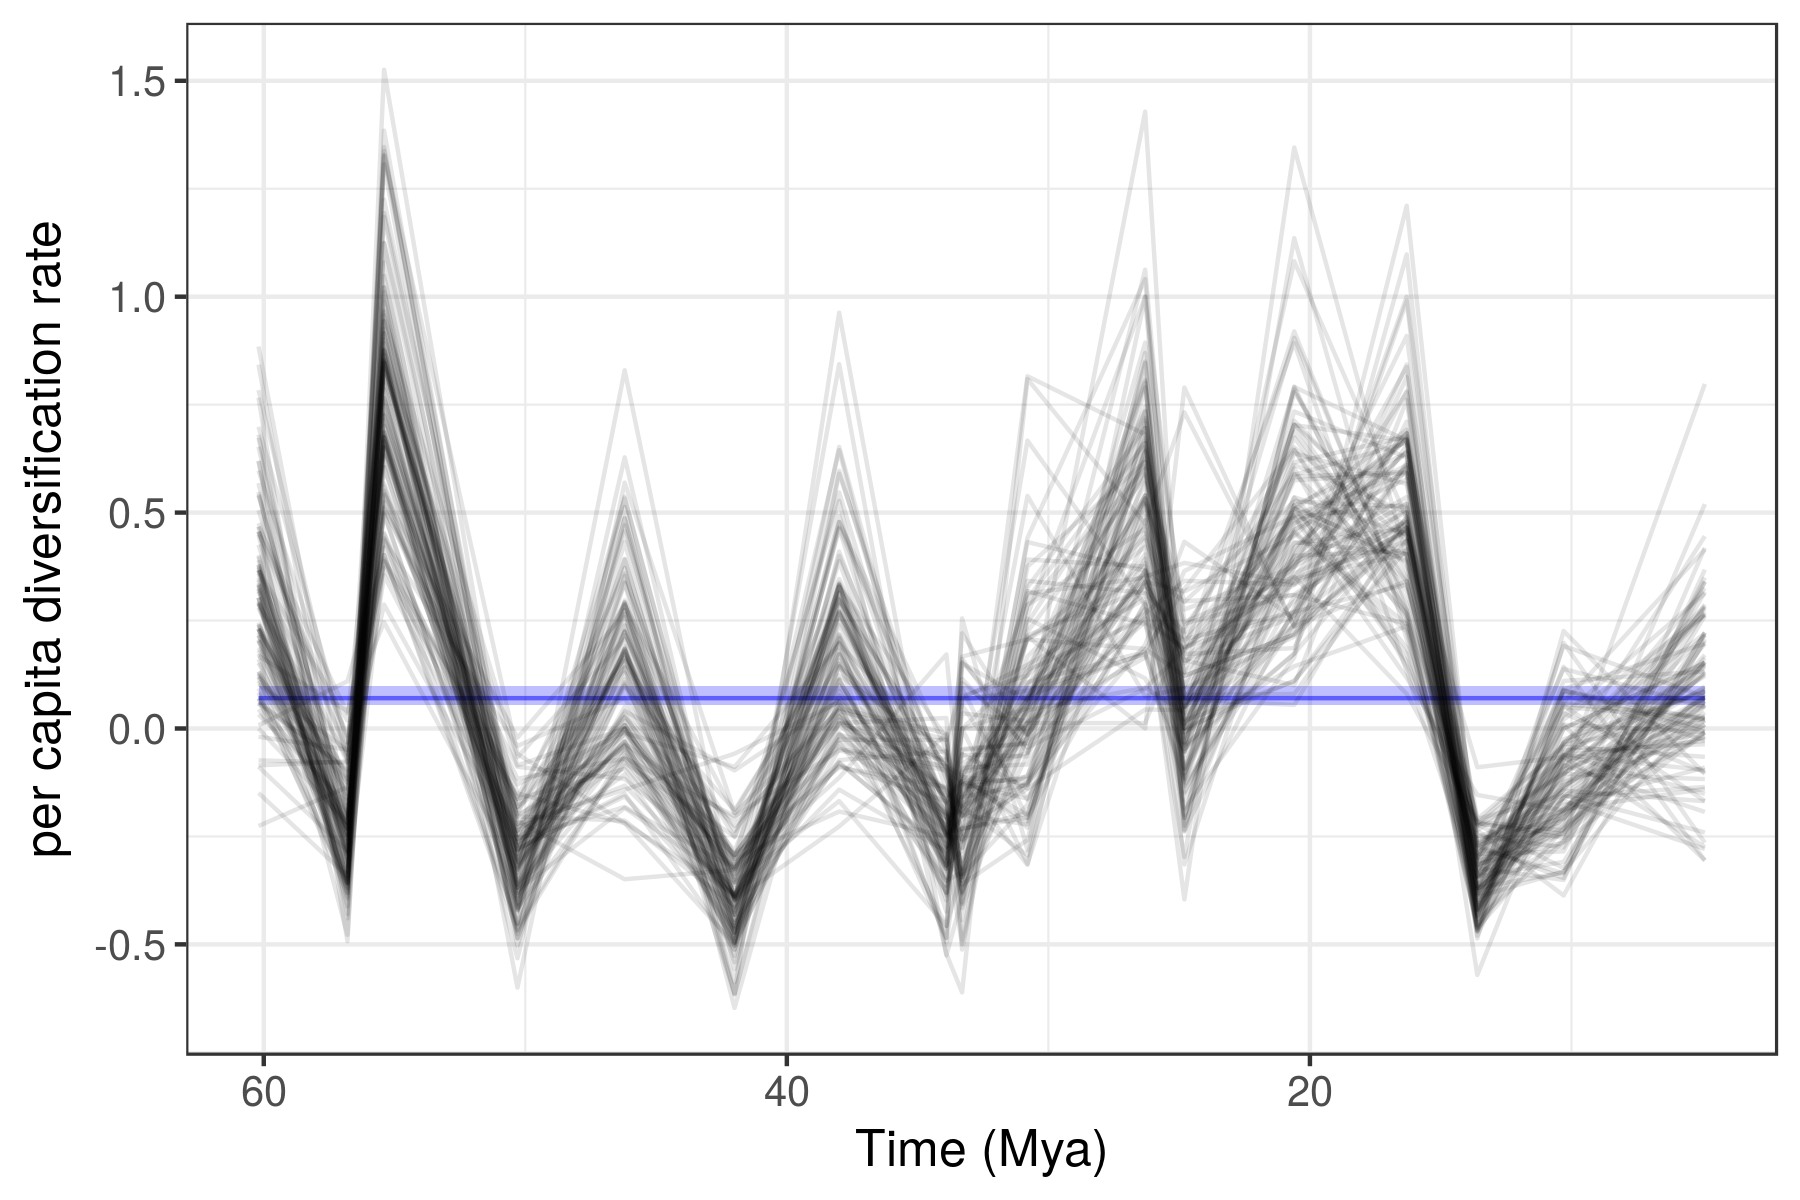
\includegraphics[width=\textwidth,height=0.8\textheight,keepaspectratio=true]{figure/div_rate}
    \caption{Diversification rate}
    %\caption[Mammal diversification rate estimates]{Posterior estimates of North American mammal diversification rate for the Cenozoic; 100 estimates are plotted to indicate the uncertainty in these estimates. As a reminder, diversification rate is the difference between origination and extinction rates and is in units of species gained per species present per time unit (2 My).}
    \label{fig:diversity_rate}
  \end{subfigure}

  \begin{subfigure}[b]{0.45\textwidth}
    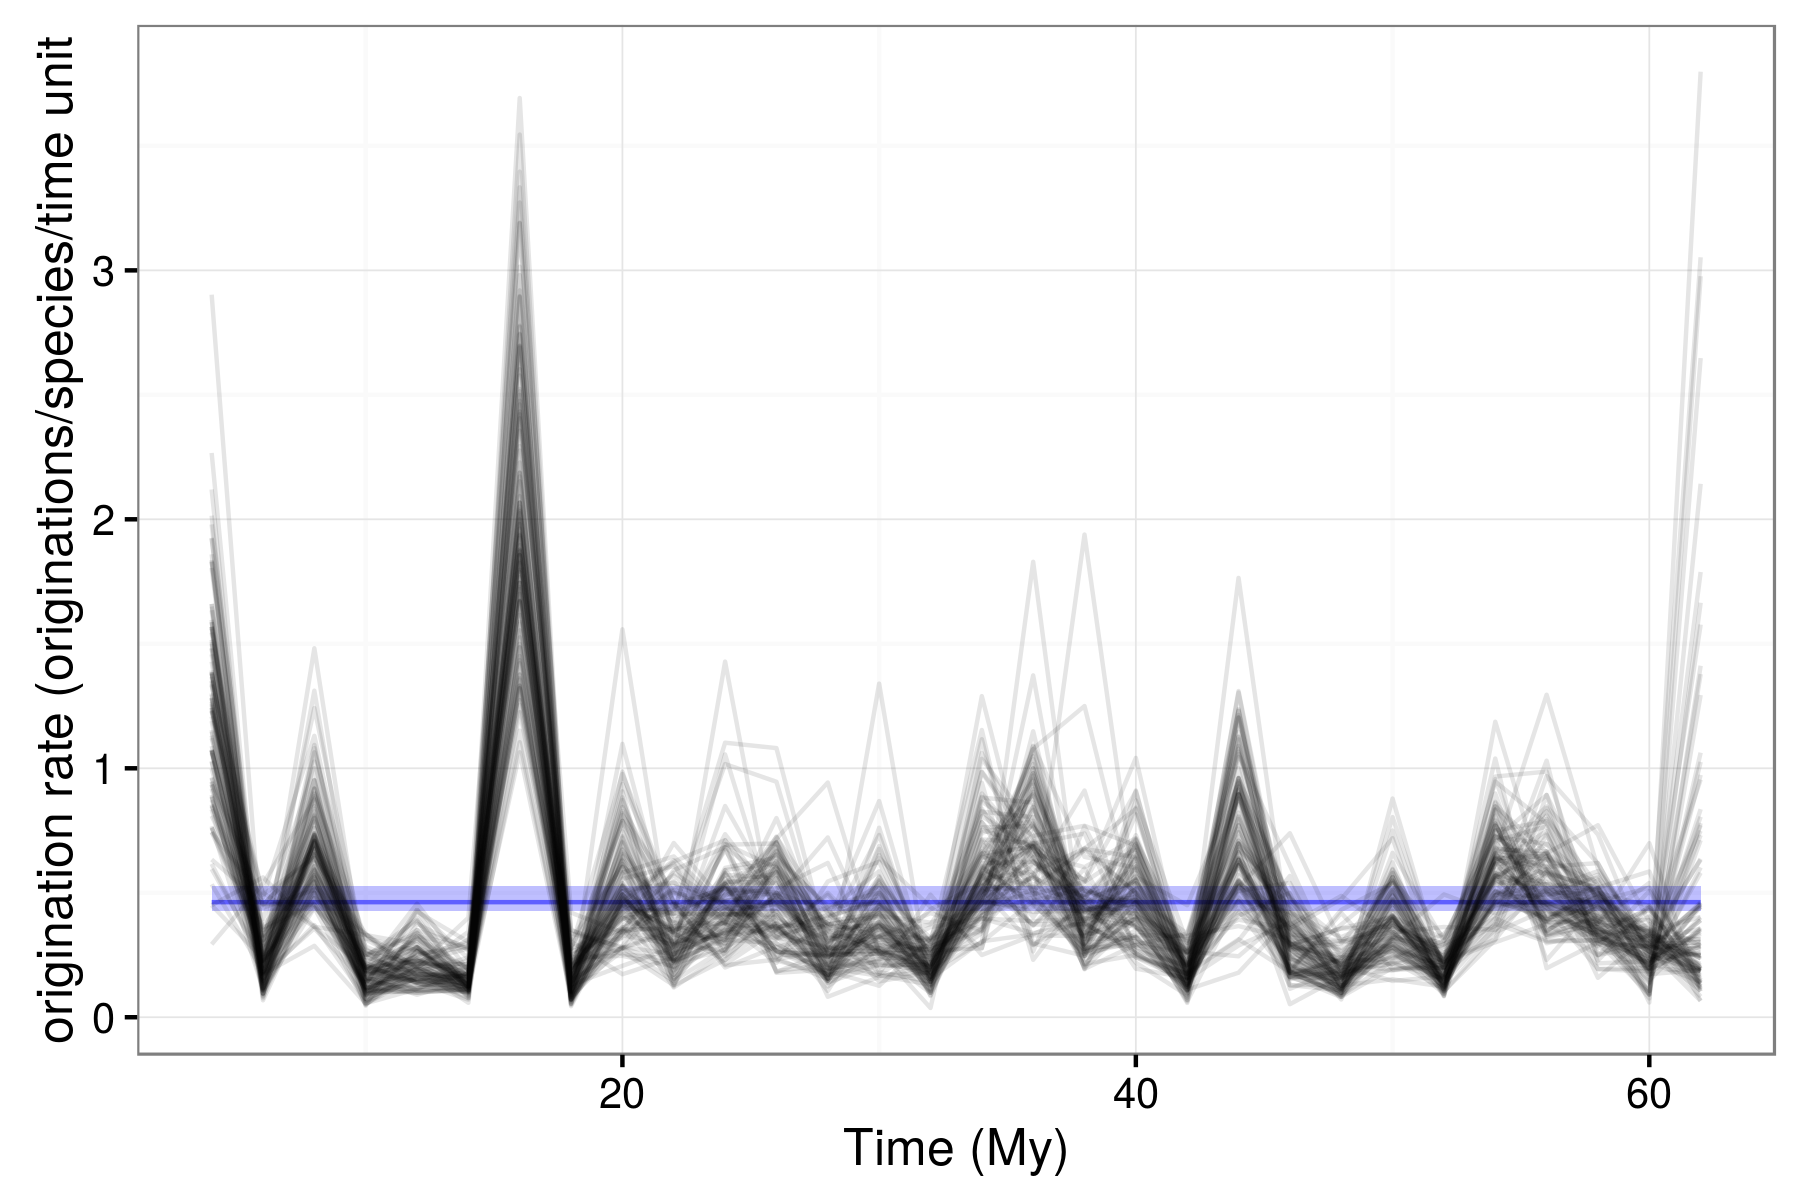
\includegraphics[width=\textwidth,height=0.8\textheight,keepaspectratio=true]{figure/orig_rate}
    \caption{Origination rate}
    %\caption[Mammal origination rate estimates]{Posterior estimates of North American origination rate for the Cenozoic; 100 estimates are plotted to indicate the uncertainty in these estimates. The unit of origination rate is number of species originating per species per time unit (2 My).}
    \label{fig:origin_rate}
  \end{subfigure}
  \begin{subfigure}[b]{0.45\textwidth}
    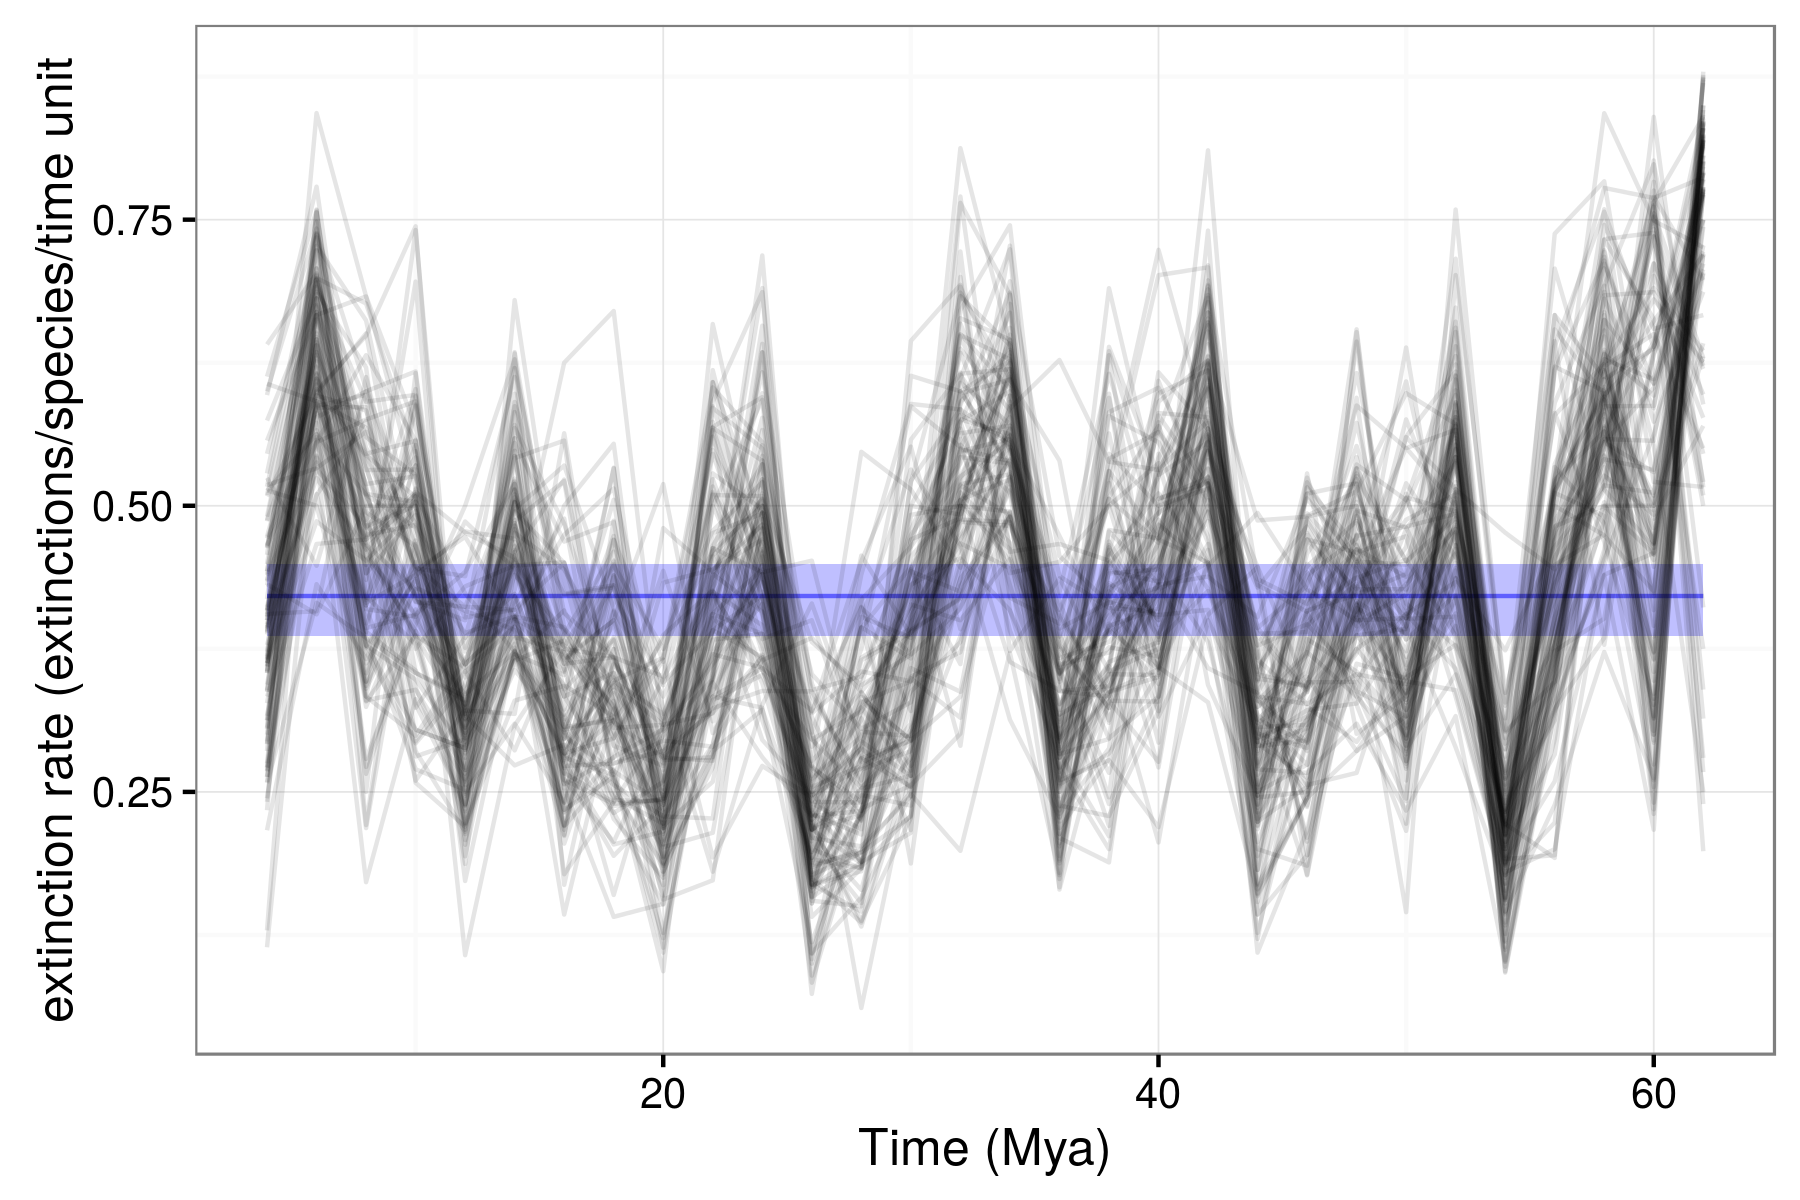
\includegraphics[width=\textwidth,height=0.8\textheight,keepaspectratio=true]{figure/death_rate}
    \caption{Extinction rate}
    %\caption[Mammal extinction rate estimates]{Posterior estimates of North American extinction rate for the Cenozoic; 100 estimates are plotted to indicate the uncertainty in these estimates. The unit of extinction rate is number of species becoming extinct per species per time unit (2 My).}
    \label{fig:extinct_rate}
  \end{subfigure}
  \caption[Estimated mammal log-diversity and macroevolutionary rates for the Cenozoic]{Posterior estimates of the time series of Cenozoic North American mammal diversity and it's characteristic macroevolutionary rates; all estimates are from the birth-death model and 100 posterior draws are plotted to indicate the uncertainty in these estimates. The dramatic differences between diversity estimates at the first and second time points and the penultimate and last time points in this series are caused by well known edge effects in discrete-time birth-death models caused by \(p_{\_, t = 1}\) and \(p_{\_, t = T}\) being partially unidentifiable \citep{Royle2008}; the hierarchical modeling strategy used here helps mitigate these effects but they are still present \citep{Gelman2013d,Royle2008}. Diversification rate is in units of species gained per species present per time unit (2 My), origination rate is in units of species originating per species present per time unit, and extinction rate is in units of species becoming extinct per species present per time unit.}
  \label{fig:macro_values}
\end{figure}




Diversity partitioned by ecotype reveals a lot of the complexity behind the pattern of mammal diversity for the Cenozoic (Fig. \ref{fig:ecotype_diversity}). 

An impressive commonality across multiple ecotype-specific diversity time series are two spikes in diversity, either up or down (Fig. \ref{fig:ecotype_diversity}). Spikes of increased diversity are seen this is seen in all arboreal ecotypes, plantigrade insectivores, scansorial insectivores, and scansorial omnivores. The converse pattern, spikes of decreased diversity, are strongly observed in the diversity history of digitigrade herbivores, with weaker decreases observed in the histories of digitigrade carnivores, and unguiligrade herbivores. % what are the similarities in group-level covariates amongst all these groups?

Arboreal ecotypes are estimated to have disappeared and reappeared as short bursts over the last 65 million years in North America, with arboreal carnivores and insectivores being most often rarer than arboreal herbivores and omnivores.

Fossorial ecotypes, whether herbivorous and insectivorous appear rare or possibly absent for most the Cenozoic, which maximum estimated diversity being obtained in the latter half of the time series (Fig. \ref{fig:ecotype_diversity}).

Plantigrade ecotypes appear most variable, plantigrade herbivores having a very different diveristy history than plantigrade carnivores and omnivores and plantigrade insectivores.

Unguligrade and plantigrade herbivores have relatively stable standing diversities throughout the Cenozoic of North America (Fig. \ref{fig:ecotype_diversity}). Similarly, digitigrade carnivorous taxa appear to have a relatively stable diversity for the Cenozoic.

\begin{figure}[ht]
  \centering
  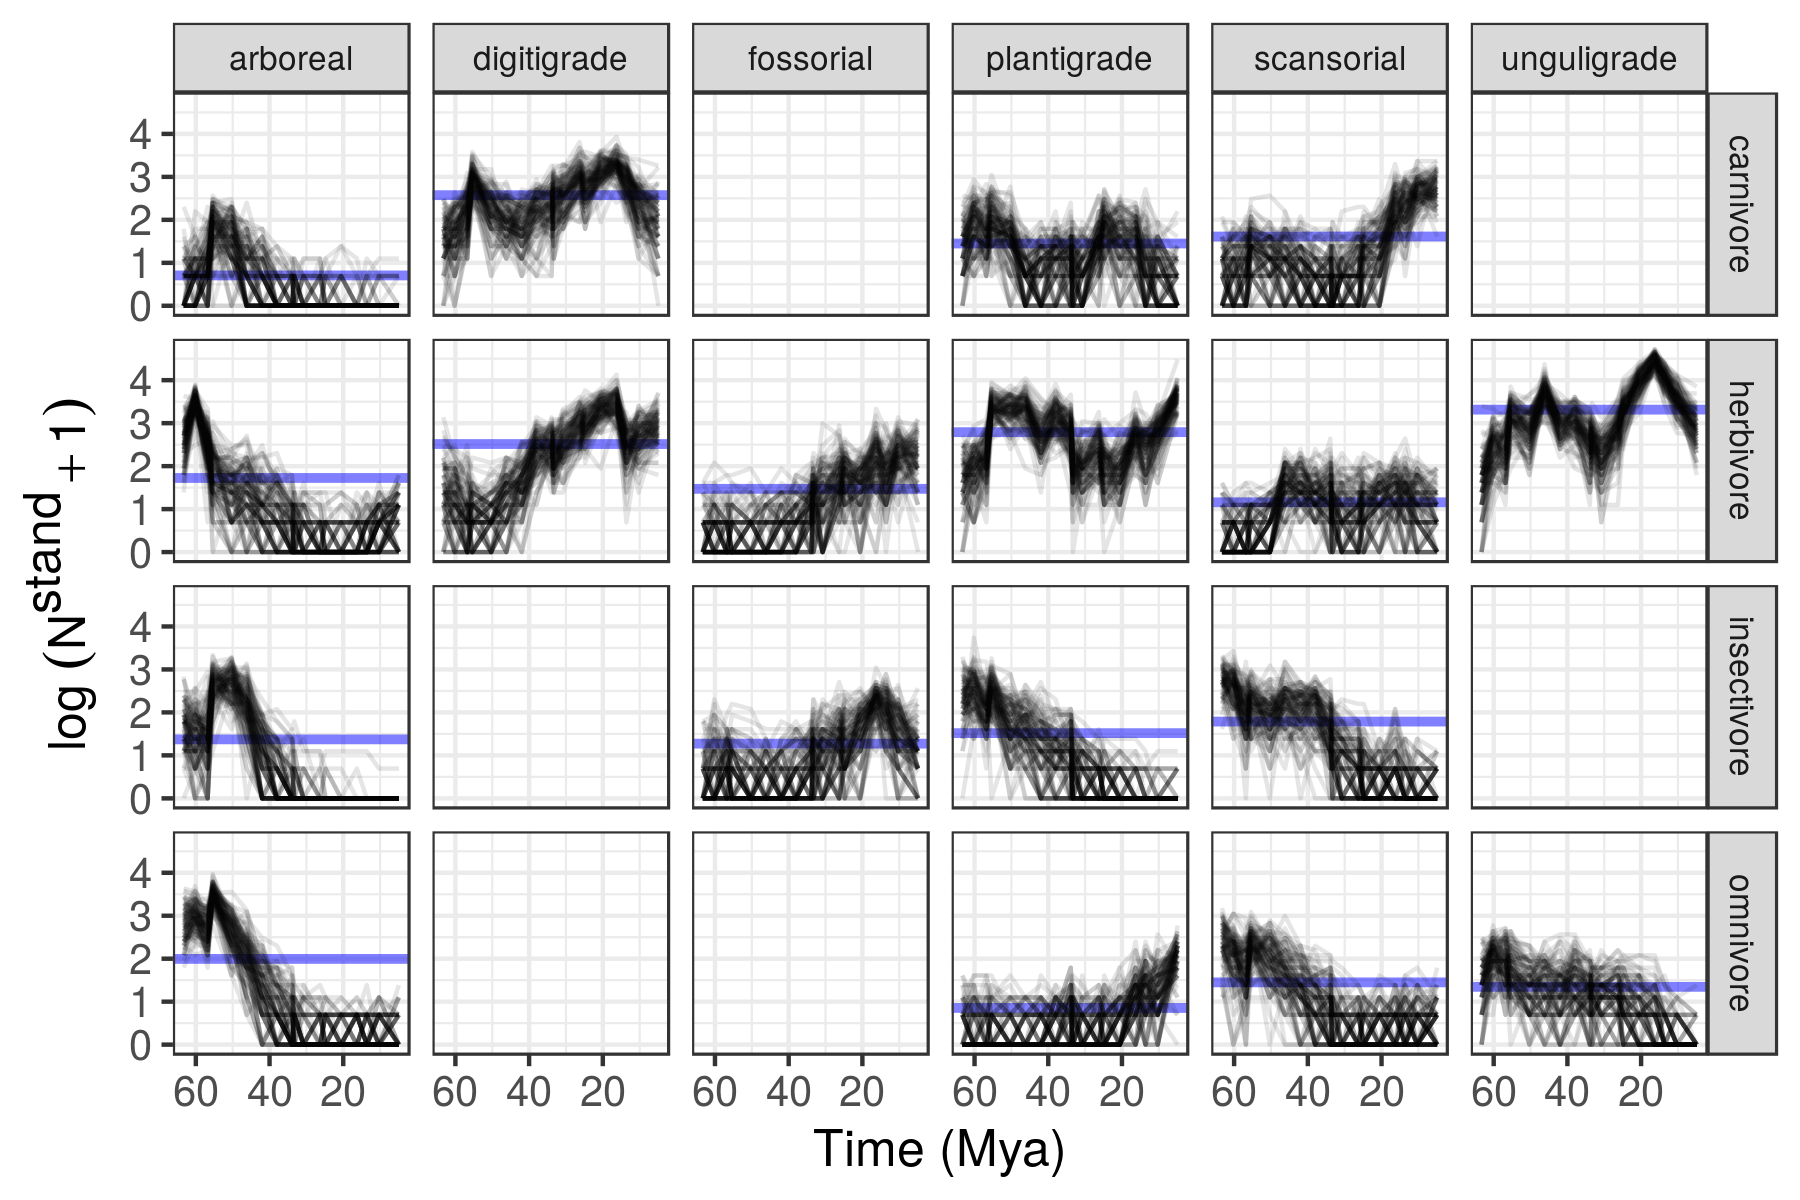
\includegraphics[width=\textwidth,height=0.8\textheight,keepaspectratio=true]{figure/ecotype_diversity}
  \caption[Estimated mammal ecotype log-diversity for the Cenozoic]{Posterior of standing log-diversity of North American mammals by ecotype for the Cenozoic as estimated from the birth-death model; 100 posterior draws are plotted to indicate the uncertainty in these estimates and what is technically plotted is log of diversity plus 1. The dramatic differences between diversity estimates at the first and second time points and the penultimate and last time points in this series are caused by well known edge effects in discrete-time birth-death models caused by \(p_{\_, t = 1}\) and \(p_{\_, t = T}\) being partially unidentifiable \citep{Royle2008}; the hierarchical modeling strategy used here helps mitigate these effects but they are still present \citep{Gelman2013d,Royle2008}.}
  \label{fig:ecotype_diversity}
\end{figure}

\end{document}
